% A Multi-Backend Predictive Framework for FIFA World Cup Fantasy Football
% Build: make all   (tectonic; see Makefile)
\documentclass[11pt,a4paper]{article}

\usepackage[margin=2.5cm]{geometry}
\usepackage{amsmath}
\usepackage{amssymb}
\usepackage{booktabs}
\usepackage{graphicx}
\usepackage{xcolor}
\usepackage[round]{natbib}
\usepackage{microtype}
\usepackage{tikz}
\usetikzlibrary{arrows.meta,positioning}
\usepackage[hidelinks]{hyperref}

\graphicspath{{../results/figures/}}

% Post-final placeholder: visible in the PDF, greppable, release-gated
% by `make final-check`.
% Provenance line at the end of every data-driven caption.
\newcommand{\figsource}[1]{\\{\footnotesize Source: \texttt{#1}}}

% Generated inline-number macros (scripts/paper_tables.py).
% GENERATED by scripts/paper_tables.py -- do not edit
\newcommand{\RmseGkHeuristic}{2.698}
\newcommand{\RmseGkPoisson}{2.491}
\newcommand{\RmseGkGbm}{2.650}
\newcommand{\RmseDefHeuristic}{3.141}
\newcommand{\RmseDefPoisson}{3.400}
\newcommand{\RmseDefGbm}{3.187}
\newcommand{\RmseMidHeuristic}{2.874}
\newcommand{\RmseMidPoisson}{4.371}
\newcommand{\RmseMidGbm}{2.767}
\newcommand{\RmseFwdHeuristic}{3.515}
\newcommand{\RmseFwdPoisson}{4.560}
\newcommand{\RmseFwdGbm}{3.153}
\newcommand{\WalkforwardPooledA}{3.164}
\newcommand{\WalkforwardPooledB}{2.952}
\newcommand{\WalkforwardPooledC}{2.724}
\newcommand{\WalkforwardPooledD}{2.735}
\newcommand{\TotalHeuristic}{325}
\newcommand{\TotalHeuristicVTwo}{340}
\newcommand{\TotalPoisson}{196}
\newcommand{\TotalGbm}{577}
\newcommand{\TotalMonteCarlo}{337}
\newcommand{\TotalEnsemble}{517}
\newcommand{\TotalUserActualNet}{240}
\newcommand{\TotalRandomBaselineMean}{105}
\newcommand{\GkRmseVOne}{2.503}
\newcommand{\GkRmseVTwo}{2.491}
\newcommand{\MarketMeanDeltaRmse}{0.703}
\newcommand{\MarketBetaTwo}{0.2}


\title{A Multi-Backend Predictive Framework for\\
       FIFA World Cup 2026 Fantasy Football}
\author{Asher Davila\\
        \small Independent Researcher\\
        \small \texttt{davilasher@gmail.com}
        \and
        Diego Guajardo\\
        \small Actuarial Scientist}
\date{July 2026}

\begin{document}

\maketitle

\begin{abstract}
We present an open-source decision-support system for the official FIFA
World Cup 2026 fantasy game, combining three expected-points backends
(a calibrated heuristic, an independent-Poisson structural model, and a
gradient-boosted tree model trained on club data), a per-position
ensemble, a mixed-integer squad optimizer, and a live decision layer,
all developed and validated during the tournament itself. Validation
is leak-free throughout, in that every model change faced a
walk-forward gate on realized tournament rounds before deployment,
and we report the failures alongside the successes. Across the seven completed rounds
the backends replayed on frozen pre-round data scored between
\TotalPoisson{} and \TotalGbm{} points against a random-squad
baseline mean of \TotalRandomBaselineMean{}, and a skill audit of
match-level forecasting found prediction-market prices losing to a
simple Elo rating out of sample, earning the market a capped minority
weight rather than the anchoring role it is usually given. The live
entry closed on \TotalUserActualNet{} net points at global rank
\GlobalRankFinal{}; its highest-scoring round was the final one, in
which a pre-committed plan holding six starters from the eventual
champion's defence, with the qualification booster active, returned
\FinalRoundNet{} points and improved the entry's global rank by
approximately 250{,}000 places. The complete system, data snapshots,
and decision log are released as open source.
\end{abstract}

\section{Introduction}
\label{sec:introduction}

Fantasy football games translate on-pitch match events into a numeric
score per player per match. The official FIFA Fantasy game for the
2026 World Cup follows the template familiar from Fantasy Premier
League: managers select a 15-player squad under a budget cap, field a
starting eleven in a valid formation, and nominate a captain whose
points are doubled; non-starters are replaced through automatic
substitutions, and per-stage rules govern transfers and the number of
players allowed from any one country. The nominal objective is to
maximise total fantasy points over the tournament. In practice most
entries also compete in a private league, which layers a ranking
objective on top of raw scoring, and the two objectives diverge in
non-trivial ways: an entry trailing the field benefits from variance,
accepting differential picks with lower expected value, while an
entry near the lead benefits from template picks that lock in the
field's expected output.

Predicting fantasy points for an international tournament is
structurally harder than the club-football problem addressed by most
prior work \citep{groos2025openfpl, mishra2025fpl}. A World Cup
compresses 104 matches into five weeks, against 380 matches over ten
months in an English Premier League (EPL) season. National teams
assemble for roughly ten days a year, so international form is
observed sparsely. The opponent distribution resembles no club
league: Argentina plays Cape Verde, not a domestic third-tier
equivalent. The group-stage cadence also induces rotation behaviour
that club play does not exhibit: a coach whose team has already
qualified rests starters on the final group matchday. A model trained
purely on club football therefore transfers imperfectly. The features
that drive club fantasy points (opponent strength, home advantage,
position-specific scoring rates) generalise; the features specific to
tournament play (manager rotation policy, top-scorer-race incentives,
knockout-stage attacking emphasis) do not exist in the club training
set at all.

The transfer problem is compounded by a hard resource constraint:
before the opening match there exist zero rows of FIFA Fantasy World
Cup 2026 training data. Our supervised learner is therefore trained
on three seasons of community-archived EPL fantasy scoring
\citep{vaastav}, \EplTrainingRows{}
player-gameweek rows in total, and international signal is injected
at inference time rather than learned. Concretely, we maintain a live
Elo rating \citep{elo1978rating, hvattum2010using, gilch2018elo}
computed over a public archive of every international match since
1872 \citep{martj42}, and the rating difference between a player's
country and its opponent enters every backend as an
opponent-strength feature.

This paper presents the system we built and then operated live for
the full tournament. Expected points are produced by an ensemble of
three backends of increasing statistical ambition: a hand-tuned
heuristic over price, position, matchup, and venue; a structural
Poisson goals model in the tradition of \citet{maher1982modelling}
and \citet{dixon1997modelling}, with positional goal and assist
shares; and a LightGBM regressor \citep{ke2017lightgbm} trained on
the EPL corpus. Squad selection, stage-aware transfer planning under
the official penalty of $-3$ points per extra transfer, and lineup
and captain choice are formulated as a mixed-integer linear
programme, solved with PuLP and the CBC solver \citep{pulp, cbc}.
The constraint set encodes the official rules stage by stage: a
\$100M budget in the group stage rising to \$105M from the round of
32, a per-country cap that relaxes from 3 to 8 as teams are
eliminated, and a rolling free-transfer allowance.

Evaluation is deliberately two-fold. Before the tournament, each
backend's per-position RMSE was measured on a held-out EPL 2024--25
end-of-season split, fixing an honest per-position choice of backend
before any World Cup data existed. During the tournament, we froze
predictions ahead of every round and logged every decision (transfer,
captain, lineup) with its rationale at decision time and its realised
outcome afterwards, including the cases in which a human domain prior
overrode the model, and whether the override was vindicated.
\POSTFINAL{headline result after the final}

This work makes the following contributions:

\begin{enumerate}
\item \textbf{System.} An end-to-end, reproducible pipeline for
  World Cup fantasy management: data collectors with schema
  validation, a per-(player, round) feature table, a three-backend
  expected-points ensemble with a live international Elo signal, and
  a MILP optimiser covering squad selection, stage-aware transfer
  planning with hit penalties, and lineup and captain choice.
\item \textbf{Cross-domain transfer.} An empirical account of
  transferring club-trained fantasy models to international
  tournament play under a zero-shot constraint, including
  per-position held-out validation used to select backends and the
  documented failure modes of the transfer, such as blindness to
  elite players without recent EPL history.
\item \textbf{In-tournament validation protocol.} A pre-registered
  style of live evaluation: predictions frozen before each round, a
  complete decision log with ex-ante rationale and ex-post outcome,
  and an explicit accounting of model recommendations versus human
  domain priors.
\item \textbf{Negative results.} We report what did not work with
  the same care as what did, including blending prediction-market
  prices into expected points \citep{benter1994computer,
  wolfers2004prediction}, a team Elo difference training feature,
  and goalkeeper defensive-form adjustments, each rejected by
  measured validation error.
\item \textbf{Open source and data.} The full codebase, frozen data
  snapshots, and generated evaluation artefacts are released
  publicly, so every table and figure in this paper can be
  regenerated from the repository
  (\POSTFINAL{repository URL once public}).
\end{enumerate}

The remainder of the paper is organised as follows.
Section~\ref{sec:related_work} reviews related work in football
modelling and fantasy points prediction. Section~\ref{sec:data}
documents the five data sources and the harmonisation required to
join them. Section~\ref{sec:methodology} develops the three predictor
backends, the Elo signal, and the MILP formulation.
Section~\ref{sec:implementation} describes the implementation and
reproducibility measures. Section~\ref{sec:validation} reports
held-out validation on the EPL split. Section~\ref{sec:live-results}
logs the live tournament round by round. Section~\ref{sec:analysis}
analyses model versus human decisions, and
Section~\ref{sec:negative-results} collects negative results.
Section~\ref{sec:lessons} distils lessons learned,
Section~\ref{sec:future_work} outlines future work, and
Section~\ref{sec:conclusion} concludes.

\section{Related Work}
\label{sec:related_work}

Our system sits at the intersection of five literatures: structural
models of goal scoring, team-strength rating systems, machine
learning for match and player outcomes, fantasy-football prediction
and squad optimisation, and the economics of betting and prediction
markets. We searched arXiv, IEEE Xplore, and ResearchGate in June
2026 for work published between 2023 and 2025 on fantasy-football
prediction, World Cup outcome modelling, and market-derived features;
coverage of the most recent quarter is limited by publication lag.
This section reviews each strand in turn, summarises the practitioner
community of practice, and closes by positioning our contributions
against the closest prior art.

\subsection{Structural models of goal scoring}
\label{sec:related-structural}

The structural approach to football match prediction models goals as
Poisson arrivals at team-level rates. \citet{maher1982modelling}
introduced the independent double-Poisson model, with each side's
scoring rate derived from latent attacking and defensive strength
parameters. \citet{dixon1997modelling} refined it with a dependence
adjustment for low-scoring matches and time-decay weighting of
historical results; notably, their work was explicitly motivated by
exploiting inefficiencies in the fixed-odds betting market, which
makes it the standard football precedent for the market-versus-model
framing we adopt in Section~\ref{sec:related-markets}.
\citet{karlis2003analysis} generalised the framework to a bivariate
Poisson model with correlated goal counts and popularised the Skellam
distribution for goal differences. The independence assumption is
empirically misspecified but only mildly so:
\citet{petretta2025dependence} report a home--away goal correlation
of $-0.085$ ($p < 0.001$) across 9{,}130 matches from the five major
European leagues, and the Dixon--Coles correction redistributes
probability mass only among the four lowest scorelines, leaving
total-goals probabilities unchanged. Our structural backend
(Section~\ref{sec:methodology}) borrows the double-Poisson shape but
replaces estimated latent strengths with observable proxies (squad
price and country Elo gap), trading a small amount of fidelity for a
model that requires no training and remains interpretable end to end.

The closest structural precedent for our tournament setting is
\citet{gilch2018elo}, who combine eloratings.net Elo covariates,
Poisson regression, and Monte Carlo simulation (100{,}000 tournament
runs) to forecast the 2018 FIFA World Cup. They backtest four Poisson
variants on the 2010 and 2014 tournaments using Brier and ranked
probability scores, find a nested Poisson specification best, and
show that freezing Elo across a simulated tournament shifts stage
probabilities by up to five percentage points in favour of stronger
teams. Their architecture anticipates ours at the team level; the
per-player fantasy-points layer, which is where the difficulty of our
problem concentrates, is absent.

Textbook treatments deserve a note on lineage.
\citet{winston2022mathletics} covers least-squares team ratings,
Poisson goal models with Skellam-based outcome probabilities (citing
\citealp{karlis2003analysis}), Elo ratings, Monte Carlo tournament
simulation, and, most relevantly, formulates daily-fantasy lineup
construction as a knapsack integer program, the direct textbook
precedent for our squad optimiser. It does not, however, engage the
Maher, Dixon--Coles, or Benter lineage at all, so we cite the primary
sources directly. \citet{eager2023football} is exclusively about
American football; we cite it only for transferable methodology:
Poisson regression for count outcomes, the stability and
regression-to-the-mean behaviour of player statistics,
simulation-based projections, and open-data reproducibility practice.

\subsection{Team-strength ratings}
\label{sec:related-ratings}

Team-strength ratings supply the fixture-difficulty signal that both
our structural and learned backends consume. The Elo system
\citep{elo1978rating} originated in chess; football adaptations add
goal-margin and match-importance multipliers and retain the
calibrated scale on which a 400-point gap corresponds to ten-to-one
odds. \citet{hvattum2010using} provide the standard evaluation of
Elo-based football forecasts against bookmaker odds: Elo carries
genuine predictive information but is less sharp than the market.
The pi-rating system of \citet{constantinou2013pi} maintains separate
home and away components updated from the predicted-versus-observed
goal-difference error, diminished through
$\psi(e) = 3\log_{10}(1+e)$; it outperformed the
\citet{hvattum2010using} Elo variants and was profitable against best
bookmaker odds over five Premier League seasons, and
\citet{bunker2024soccer} confirm that pi-ratings beat Elo on
goal-difference-aware tasks. The same authors later extended this
rating-driven line to long-term team performance modelling
\citep{constantinou2017towards}. We nonetheless use Elo: it is
simpler to roll forward from open match histories, easier to falsify,
and the home--away asymmetry at the heart of pi-ratings matters less
at a World Cup played almost entirely on neutral ground. The FIFA
Men's World Ranking, the governing body's monthly official ranking,
is less responsive to recent form than Elo and serves only as a
fallback in our system (Section~\ref{sec:data}).

\subsection{Machine learning for match and player outcomes}
\label{sec:related-ml}

\citet{bunker2024soccer} demonstrate that gradient-boosted tree
models trained on engineered rating features (pi-ratings, Elo,
momentum) currently set the state of the art for club-football match
outcome prediction across multiple European leagues. For the
international tournament setting, recent work integrates team-level
and player-specific metrics with dimensionality reduction and
validates on the 2022 World Cup, finding that player attributes
combined with team composition improve outcome accuracy
\citep{worldcup2025players}; it does not address fantasy-points
prediction or the club-to-country transfer problem we tackle. A related recent line forecasts full
goal-difference distributions rather than point estimates,
% TODO cite: distributional Skellam forecasting preprint (2025)
which our player-level quantile heads capture in part. A systematic
review of machine learning in sports betting
\citep{sportsbetting2024review} identifies distribution shift between
training and live data as a recurring failure mode across the field;
the model variant we rejected for exactly this reason
(Section~\ref{sec:negative-results}) is an instance of the pattern.

At the player-regression level our problem is small-scale tabular
learning. Gradient-boosted decision trees, LightGBM
\citep{ke2017lightgbm} and XGBoost \citep{chen2016xgboost} in
particular, dominate small-to-mid tabular benchmarks, and systematic
comparisons find that they consistently beat neural networks on
tabular data at moderate scale \citep{borisov2022deeptabular,
shwartz2022tabular}. We use LightGBM for three practical reasons:
native handling of missing values in features that exist at inference
time but not in training, deterministic training under fixed seeds
(which makes feature A/B tests meaningful), and fast CPU-only
training and scoring with no model-serving runtime. We deliberately
do not use neural networks: our labelled table
(Section~\ref{sec:data}) is orders of magnitude below the data scale
at which deep models earn their keep, each row carries only five
features with no hierarchical structure for representation learning
to exploit, and a tree ensemble stored as plain text can be inspected
feature by feature.

\subsection{Fantasy-football prediction and squad optimisation}
\label{sec:related-fantasy}

Fantasy Premier League (FPL) supports a large public modelling
community, and its accumulated conventions inform our design:
position-specific models outperform pooled models, recent form is the
strongest single feature, fixture difficulty is the second, and
quantile predictions are useful for differential strategies. We adopt
all four: one model per position, form features in two of our
backends, an Elo fixture-difficulty term, and quantile heads at the
10th, 50th, and 90th percentiles.

The closest published comparable to our system is OpenFPL
\citep{groos2025openfpl}: position-specific ensembles trained on FPL
and Understat data from 2020--21 through 2023--24 and validated
prospectively on 2024--25, achieving accuracy comparable to a leading
commercial service and outperforming it on high-return players (above
two points), with models and inference code released openly. The
architectural overlap with our work is substantial: position-specific
models, multi-gameweek horizons, and open-source publication. We
differ in five respects: (i) we target an international tournament
rather than a club season; (ii) we run three explicit backends
(heuristic, structural Poisson, gradient-boosted trees) and select
the best per position on held-out validation, where their ensemble is
opaque about which member dominates where; (iii) we integrate a live
international Elo rolled from an independent match-history archive
\citep{martj42}; (iv) we couple prediction to a stage-aware
mixed-integer optimiser with transfer-hit accounting, where OpenFPL
addresses prediction accuracy only; and (v) we publish a
user-in-the-loop decision log.

On the optimisation side, \citet{mishra2025fpl} formulate starting
eleven, bench, and captain selection as mixed-integer linear programs
under FPL's budget, formation, and per-club constraints, and report
that ARIMA performs best among their point predictors. Their
optimisation formulation is close to ours; their prediction component
is simpler (a single model, no quantiles, no structural backend).
Beyond these, transformer-based sentiment analysis of player news has
been combined with statistical features to improve FPL point
prediction,
% TODO cite: sentiment-enriched FPL prediction (ResearchGate, 2025)
an idea our team-news roadmap (Section~\ref{sec:future_work}) adapts
to the international setting, and earlier baseline studies applied
linear models, decision trees, and random forests to FPL scoring.
% TODO cite: Bangaru et al. (2022), IEEE

\subsection{Prediction markets and the favourite-longshot bias}
\label{sec:related-markets}

The seminal work on combining a fundamental model with public market
signals is \citet{benter1994computer}. Benter trained a logit-based
handicapping model on horse-race data and showed that its residual,
after conditioning on the parimutuel market's implied probabilities,
still carried predictive signal: a model that beats the public must
combine its own features with the public's information rather than
replace it. Prediction markets more broadly aggregate dispersed
information into prices with well-documented forecasting accuracy
\citep{wolfers2004prediction}.

Treating market prices as direct probability estimates is
nevertheless naive. \citet{thaler1988favorite} document the
favourite-longshot bias in horse racing: casual bettors
systematically underbet favourites and overbet longshots, producing
predictable inefficiencies that sharp money arbitrages but does not
eliminate. \citet{snowberg2010explaining} test competing explanations
and attribute the bias to misperception of small probabilities rather
than risk-loving preferences. \citet{levitt2004sportsbook} shows that
sportsbooks price to exploit bettor biases rather than to balance
their books: in his sample, favourites covered the point spread in
only 49.1\% of games even though bettors overwhelmingly backed them.
\citet{croxson2014information} show that market efficiency varies
with liquidity, with in-play football prices incorporating goal news
swiftly in liquid markets while thin markets carry larger biases.
The implication for our methodology is that market prices are noisy
probability estimators whose noise mixes information aggregation
(signal) with behavioural bias (anti-signal); the appropriate
response is neither to treat them as ground truth nor to discard
them, but to combine them with a fundamental model using empirically
estimated weights, exactly as \citet{benter1994computer} did for
parimutuel racing.

We could find no published academic work that uses contemporary
prediction-market venues such as Polymarket or Kalshi as a feature
source for fantasy-football prediction, despite both venues listing
contracts directly relevant to fantasy decisions: match outcomes,
first and anytime goalscorers, and tournament top scorer. Updating
the Benter combining approach for these markets and applying it to
FIFA fantasy is, to our knowledge, new; we develop the proposal in
Section~\ref{sec:future_work}.

\subsection{Practitioner practice}
\label{sec:related-practice}

Alongside the academic literature sits a large community of practice:
editorial and analytics sites such as Fantasy Football Scout, Fantasy
Football Hub, and AllAboutFPL, tooling platforms such as Premier
Fantasy Tools and FPL Copilot, and data-science write-ups from
consultancies such as Frontier Economics.
% TODO cite: Frontier Economics FPL strategy analysis (web)
The practitioner consensus on captaincy, the highest-leverage
decision per round, is to rank by expected points, anchor on recent
form, weight fixture difficulty heavily, monitor rotation and injury
risk through pre-match press conferences, and condition differential
strategy on league position: managers who lead should match the
consensus pick, while chasing managers should take one or two
low-ownership picks, with returns diminishing beyond two. Published
booster-timing guides for the World Cup 2026 format make analogous
recommendations at the chip level.

Our system encodes much of this consensus directly (expected-points
ranking, form anchoring, an Elo fixture-difficulty term, vice-captain
as the second-highest projection), so the difference is
methodological rather than tactical: we impose held-out validation
gates before shipping a backend, compare backends systematically,
optimise under formal constraints rather than editorial tiers,
propose market integration, and keep a decision log that records
model recommendation, human override, and realised outcome. The
practitioner sites deliver excellent weekly advice for their
audience; what they do not do is measure their own cumulative
accuracy in a way that later work can build on.

\subsection{Positioning against prior art}
\label{sec:related-positioning}

Table~\ref{tab:contributions-prior-art} draws the line between prior
art and this paper's contributions.

\begin{table}[t]
\centering
\small
\begin{tabular}{@{}p{0.24\linewidth}p{0.28\linewidth}p{0.40\linewidth}@{}}
\toprule
Contribution & Closest prior art & Our delta \\
\midrule
MILP squad and captain selection &
\citet{mishra2025fpl}; knapsack formulation in
\citet{winston2022mathletics} &
Stage-aware constraints (group versus knockout), transfer-hit
accounting, three-backend prediction input \\
\addlinespace
Position-specific predictors &
\citet{groos2025openfpl}; \citet{bunker2024soccer} &
Three explicit backends with per-position selection on held-out
validation, rather than an opaque ensemble \\
\addlinespace
Club-to-country transfer &
None published &
Train on club fantasy data, infer on the World Cup; document the
distribution-shift failure modes \\
\addlinespace
Live international Elo in fantasy &
\citet{hvattum2010using} &
Elo rolled from an open match archive \citep{martj42} and
prioritised over the static FIFA ranking \\
\addlinespace
Prediction-market features &
\citet{benter1994computer} &
Polymarket and Kalshi prices proposed as a feature source for FIFA
fantasy \\
\addlinespace
Ownership-aware captaincy &
None &
Monte Carlo captain selection that models the field's likely
captain distribution \\
\addlinespace
User-in-the-loop decision log &
None &
Per-round record of model recommendation, human override, and
realised outcome \\
\bottomrule
\end{tabular}
\caption{Our contributions against the closest prior art.}
\label{tab:contributions-prior-art}
\end{table}

In short, each component of our system has a clear ancestor: the
Poisson lineage of \citet{maher1982modelling} and
\citet{dixon1997modelling}, the Elo evaluation of
\citet{hvattum2010using}, the tournament simulation of
\citet{gilch2018elo}, the fantasy prediction of
\citet{groos2025openfpl}, the fantasy optimisation of
\citet{mishra2025fpl}, and the market combining of
\citet{benter1994computer}. What has not appeared before is their
combination in a single validated pipeline for an international
tournament, run live under real transfer deadlines, with its
decisions and failures documented.

\section{Data}
\label{sec:data}

Our system draws on six data sources: the official FIFA Fantasy API
(the primary inference source), a public archive of international
match results \citep{martj42}, club-level match and odds data
\citep{footballdata}, community dumps of English Premier League
fantasy scoring \citep{vaastav}, a static copy of the FIFA Men's
World Ranking as a fallback, and a community-maintained World Cup
2026 statistics dataset \citep{mominul2026dataset} providing real
match expected goals, lineups with minutes, and referee card
histories. This section describes each source, the schemas we
consume, and the harmonisation work required to join them.

\subsection{FIFA Fantasy API}
\label{sec:data-fifa-api}

The primary inference source consists of three JSON endpoints under
\texttt{play.fifa.com/json/fantasy/}:

\begin{itemize}
\item \texttt{players.json}: one record per player, with \texttt{id},
  position, price (in millions), \texttt{percentSelected} (ownership,
  0--100), \texttt{status} (playing, transferred, and similar),
  \texttt{oneToWatch}, and a \texttt{stats} block containing
  \texttt{totalPoints}, \texttt{lastRoundPoints}, \texttt{form},
  \texttt{roundPoints}, and \texttt{nextFixtureFromActiveRound}.
\item \texttt{squads.json}: one record per national team, with
  \texttt{id}, \texttt{name}, \texttt{abbr}, \texttt{group}, and
  \texttt{isEliminated}.
\item \texttt{rounds.json}: one record per round, with status, start
  and end dates, and a \texttt{tournaments} array of fixtures (home
  and away squad ids, kickoff time, and scores once played).
\end{itemize}

\paragraph{Schema drift at MD1 kickoff.}
Pre-tournament, \texttt{stats.roundPoints} was a list of integers. On
the day Matchday~1 started, the field switched to a dictionary keyed
by round id (for example \texttt{\{"1": 7\}}). Our Pydantic schema
initially modelled the field as a list, which broke the parser at the
worst possible moment. The fix accepts both shapes via a
\texttt{list[int] | dict[str, int]} union type and a normaliser that
emits a list indexed by round position, so downstream code is
insulated from the representation.

\paragraph{Two-stage validation.}
A first layer of raw Pydantic models mirrors the API verbatim
(camelCase field names, all-optional wherever the source is
unreliable). A second normalisation pass produces the downstream
contract (\texttt{Squad}, \texttt{Player}, \texttt{Fixture}) consumed
by every later module. This is the standard anti-corruption-layer
pattern: the API can drift without breaking the rest of the codebase,
provided only the normalisation pass is updated.

\subsection{International match results and live Elo}
\label{sec:data-elo}

We consume a public CSV of every international match since 1872
\citep{martj42}, with columns \texttt{date}, \texttt{home\_team},
\texttt{away\_team}, \texttt{home\_score}, \texttt{away\_score},
\texttt{tournament}, \texttt{city}, \texttt{country}, and
\texttt{neutral}. The companion goalscorer and shootout files exist
but we do not consume them.

From this history we compute an Elo rating \citep{elo1978rating} per
country by rolling forward through the date-sorted match list. The
K-factor varies by tournament weight: 60 for World Cup matches, 25
for qualifiers, and 10 for friendlies. A goal-margin adjustment
scales the K-factor by $\sqrt{(m+1)/2}$ for a margin of $m$ goals,
and home advantage adds 60 to the home side's expected score except
in neutral fixtures; both choices follow common practice in
Elo-based football forecasting \citep{hvattum2010using}. The output
table holds, per country, the current Elo, match count, form over the
last ten matches, goals for and against over the trailing 24 months,
and the date of the most recent match.

\subsection{Club-level enrichment}
\label{sec:data-clubs}

We download per-league, per-season CSVs from football-data.co.uk
\citep{footballdata} for the top five European leagues (Premier
League, La Liga, Bundesliga, Serie A, Ligue 1), covering the most
recent three full seasons plus earlier seasons used only as Elo seed
data. The data serves three purposes:

\begin{itemize}
\item a per-club Elo rating, computed analogously to the
  international Elo above;
\item a normalised match table carrying bookmaker closing odds
  (Pinnacle, with Bet365 as fallback) where available;
\item a per-club, per-date Elo timeline used to attach
  team-Elo-at-match-time to the Premier League training rows without
  lookahead bias.
\end{itemize}

\subsection{Premier League fantasy dumps as training data}
\label{sec:data-fpl}

Labelled training data comes from a public mirror of every English
Premier League fantasy round \citep{vaastav}. We ingest three full
seasons (2022--23, 2023--24, 2024--25) into per-player, per-gameweek
Parquet tables. After dropping non-appearances (zero-minute rows), we
retain \EplTrainingRows{} labelled rows across
the three seasons.

\subsection{Static FIFA World Ranking fallback}
\label{sec:data-rankings}

We also maintain a static copy of the FIFA Men's World Ranking,
hand-transcribed from FIFA's own publication. It serves as a fallback
for the country-strength feature when the live Elo of
Section~\ref{sec:data-elo} is unavailable, mostly for countries that
have not played any international match within the cached window. The
heuristic and Poisson backends prefer Elo over the static rank when
both are present, fall back to the rank when Elo is missing, and fall
back to a price-only signal when neither is present.

\subsection{Country-name harmonisation}
\label{sec:data-names}

A persistent integration cost is that each source spells country
names differently: United States versus USA versus United States of
America, or Korea Republic versus South Korea. A hand-maintained
mapping table holds canonical lookups in two directions: one mapping
used when joining the international Elo into the per-player feature
table, and one mapping club names between the fantasy dumps and the
club-level match data. Three near-misses had to be fixed during
integration: Bosnia and Herzegovina (both sources agree, but our
initial mapping incorrectly rewrote it); Czechia (FIFA) versus Czech
Republic in the match archive; and T\"urkiye (FIFA, the country's
official name since 2022) versus Turkey. Each was caught by an
after-join NaN scan over the country-Elo column of the per-player,
per-round feature table.

\section{Methodology}
\label{sec:methodology}

Our system is a pipeline of five stages. A feature builder joins the
data sources of Section~\ref{sec:data} into one table with a row per
(player, upcoming round). Three expected-points backends, a calibrated
heuristic, a structural independent-Poisson model, and a
gradient-boosted tree model, score that table independently; an
experimental Monte Carlo simulator provides a fourth, distributional
view. A per-position ensemble routes each position to the backend that
wins it on held-out data. A rule-encoding step converts predictions
into effective points, and a mixed-integer optimiser selects squads,
transfers, and lineups. Finally, a live layer supports the in-play
decisions the game allows after kickoff. This section specifies each
stage; formal statements of the optimisation programs and auxiliary
algorithms appear in Appendix~\ref{sec:b}.

Throughout, $i$ indexes a (player, round) row, $\pi(i) \in
\{\mathrm{GK}, \mathrm{DEF}, \mathrm{MID}, \mathrm{FWD}\}$ is the
player's position, $p_i$ is the price in millions, and $h_i \in \{0,
1\}$ indicates a home fixture. All backends share an availability
contract: a player whose status is not \emph{playing}, whose squad is
eliminated, or whom confirmed team news places on the bench is
predicted at zero.

\subsection{Per-player, per-round feature contract}
\label{sec:methodology-features}

The feature table contains one row per player per upcoming round in
which their squad plays. Its columns fall into five groups:

\begin{itemize}
\item \textbf{Player metadata:} identity, position, country, price,
  ownership fraction, availability status, an elimination flag, and
  the realised scoring history (cumulative points, last-round points,
  per-round points, and the game's own form value).
\item \textbf{Fixture context:} round, stage, kickoff time, home flag,
  opponent identity, and venue.
\item \textbf{Own-squad strength:} total and average squad price, and
  the mean price of the squad's top eleven players by price
  (\texttt{squad\_top\_n\_avg\_price}), which we use as a proxy for
  first-team strength.
\item \textbf{Opponent strength:} the same columns for the opposing
  squad, prefixed \texttt{opp\_}.
\item \textbf{Derived:} the top-eleven price gap
  (\texttt{strength\_diff}), the FIFA ranking gap
  (\texttt{rank\_diff}), the rolling country Elo of both sides and
  their difference (Section~\ref{sec:data-elo}), last-ten-match
  national-team form, and rest-day counts to the previous and next
  match.
\end{itemize}

The table is intentionally over-wide: each backend consumes only the
subset it needs, and adding a candidate feature never requires a
schema change downstream. Opponent strength is deliberately
first-class; fixture difficulty enters every backend rather than
being an afterthought.

\subsection{Backend 1: calibrated heuristic}
\label{sec:methodology-heuristic}

The first backend is a hand-calibrated formula with no training step.
Each row receives

\begin{equation}
\hat{y}_i \;=\; c_{\pi(i)}\, p_i
  \left(1 + \alpha \tanh z_i\right)
  \left(1 + \beta\, h_i\right)
  \;+\; \gamma \max\!\left(0,\; p_i - 9.0\right),
\label{eq:heuristic}
\end{equation}

where $c_{\pi}$ is a per-position points-per-price coefficient
($c_{\mathrm{GK}} = 0.50$, $c_{\mathrm{DEF}} = 0.55$,
$c_{\mathrm{MID}} = 0.60$, $c_{\mathrm{FWD}} = 0.65$), $\alpha = 0.40$
saturates the matchup adjustment at $\pm 40$\,\%, $\beta = 0.05$ is a
home boost, and $\gamma$ is a premium-tier boost above the 9.0M price
threshold, zero by default. The matchup signal $z_i$ blends a
price-based strength gap with the best available national-team
strength signal:

\begin{equation}
z_i =
\begin{cases}
0.35\, z^{\mathrm{price}}_i + 0.65\, z^{\mathrm{elo}}_i
  & \text{if country Elo is available,}\\[2pt]
0.35\, z^{\mathrm{price}}_i + 0.65\, z^{\mathrm{rank}}_i
  & \text{else if a FIFA ranking is available,}\\[2pt]
z^{\mathrm{price}}_i & \text{otherwise,}
\end{cases}
\label{eq:heuristic-z}
\end{equation}

with $z^{\mathrm{price}}_i = \Delta^{\mathrm{price}}_i / 2$,
$z^{\mathrm{elo}}_i = \Delta^{\mathrm{elo}}_i / 400$, and
$z^{\mathrm{rank}}_i = \Delta^{\mathrm{rank}}_i / 250$, where
$\Delta^{\mathrm{price}}$ is the top-eleven price gap,
$\Delta^{\mathrm{elo}}$ the country Elo gap, and
$\Delta^{\mathrm{rank}}$ the FIFA ranking-points gap. The divisors
normalise each signal to a comparable scale; 400 Elo points is the
rating system's natural one-tier distance \citep{elo1978rating}. The
Elo signal takes priority because it is derived live from realised
international results \citep{hvattum2010using}; the static ranking is
the fallback, and club-price alone carries the signal when neither is
present (as in club-league training data).

The heuristic's strengths are transparency and robustness: every
constant is explainable, no training data is required, and there is
no distribution-shift risk between club and tournament data. Its
weakness is that it cannot learn. If a real pattern exists that the
formula does not encode, the heuristic will never find it, and its
linear-in-price base term flattens the true, non-linear marginal
return of premium players. An attempt to graft a fixed-weight
realised-form blend onto this formula lost to the unmodified version
in every backtested round (Section~\ref{sec:negative-results}), which
informed the design of the learned form feature in
Section~\ref{sec:methodology-gbm}.

\subsection{Backend 2: structural Poisson model}
\label{sec:methodology-poisson}

The second backend follows the independent-Poisson tradition of
football score modelling \citep{maher1982modelling,
dixon1997modelling}: estimate each team's expected goals, distribute
them across positions, and map the result to fantasy points through
the official scoring rules. Like the heuristic it requires no
training data.

\paragraph{Step 1: team expected goals.}
A matchup score combines the available strength signals,

\begin{equation}
m_i = s_i + \frac{\Delta^{\mathrm{price}}_i}{6},
\qquad
s_i =
\begin{cases}
\Delta^{\mathrm{elo}}_i / 400 & \text{if Elo is available,}\\[2pt]
\Delta^{\mathrm{rank}}_i / 800 & \text{else if a ranking is
  available,}\\[2pt]
0 & \text{otherwise,}
\end{cases}
\label{eq:poisson-matchup}
\end{equation}

and maps to expected goals for the player's team and its opponent
through a clipped exponential around a base rate of 1.30 goals per
team per match, with a 10\,\% boost for the home side:

\begin{align}
\lambda^{\mathrm{own}}_i &= 1.30\,
  e^{\operatorname{clip}(m_i,\, [-1.2,\, 1.2])}
  \left(1 + 0.10\, h_i\right),
\label{eq:poisson-own}\\
\lambda^{\mathrm{opp}}_i &= 1.30\,
  e^{-\operatorname{clip}(m_i,\, [-1.2,\, 1.2])}
  \left(1 + 0.10\, (1 - h_i)\right).
\label{eq:poisson-opp}
\end{align}

Clipping the exponent keeps predictions sane for extreme mismatches.

\paragraph{Step 2: positional distribution.}
Team expected goals are distributed across positions with fixed
shares (Table~\ref{tab:poisson-constants}): a player's expected goals
are $\lambda^{\mathrm{own}}_i\, s^{G}_{\pi(i)}$ and, taking roughly
70\,\% of goals to carry an assist, expected assists are $0.7\,
\lambda^{\mathrm{own}}_i\, s^{A}_{\pi(i)}$.

\begin{table}[t]
\centering
\caption{Poisson backend constants per position: goal share $s^{G}$,
assist share $s^{A}$, points per goal $G$, and clean-sheet points
$C$. Point values follow the official game rules.}
\label{tab:poisson-constants}
\begin{tabular}{lcccc}
\toprule
Position & $s^{G}$ & $s^{A}$ & $G$ & $C$ \\
\midrule
GK  & 0.00 & 0.01 & 9 & 5 \\
DEF & 0.10 & 0.18 & 7 & 5 \\
MID & 0.30 & 0.50 & 6 & 1 \\
FWD & 0.50 & 0.31 & 5 & 0 \\
\bottomrule
\end{tabular}
\end{table}

\paragraph{Step 3: defensive terms.}
Under the Poisson assumption the clean-sheet probability is exact,
$P(\text{clean sheet}) = e^{-\lambda^{\mathrm{opp}}_i}$, and the
expected goals conceded beyond the first, which the rules penalise,
has the closed form

\begin{equation}
\xi_i = \mathbb{E}\bigl[\max(0,\, K - 1)\bigr]
      = \lambda^{\mathrm{opp}}_i - 1 + e^{-\lambda^{\mathrm{opp}}_i},
\qquad K \sim \mathrm{Poisson}\bigl(\lambda^{\mathrm{opp}}_i\bigr).
\label{eq:poisson-xi}
\end{equation}

\paragraph{Step 4: expected fantasy points.}
The components sum, with a 2-point appearance baseline, 3 points per
assist, a goalkeeper save bonus scaling at 0.50 points per unit of
opponent expected goals (an empirically calibrated constant; the
value derived from first principles measured worse, see
Section~\ref{sec:negative-results}), and the conceded-goals penalty
applied fully to goalkeepers and at rate 0.5 to defenders:

\begin{align}
\hat{y}_i = \max\Bigl(0,\;
  & 2
  + \lambda^{\mathrm{own}}_i\, s^{G}_{\pi(i)}\, G_{\pi(i)}
  + 3 \cdot 0.7\, \lambda^{\mathrm{own}}_i\, s^{A}_{\pi(i)}
  + e^{-\lambda^{\mathrm{opp}}_i}\, C_{\pi(i)} \nonumber\\
  & + \mathbf{1}\bigl[\pi(i) = \mathrm{GK}\bigr]
      \bigl(0.50\, \lambda^{\mathrm{opp}}_i - \xi_i\bigr)
    - \mathbf{1}\bigl[\pi(i) = \mathrm{DEF}\bigr]\, 0.5\, \xi_i
  \Bigr).
\label{eq:poisson-total}
\end{align}

Every term traces to a single football statement, and the clean-sheet
term is exact under the model. The weaknesses are the independence
assumption itself, which ignores score correlation between the two
teams \citep{karlis2003analysis}, and the population-average shares:
the model cannot tell a star striker from his backup if they share a
price and a matchup.

\subsection{Backend 3: gradient-boosted trees}
\label{sec:methodology-gbm}

The third backend is a LightGBM model \citep{ke2017lightgbm} per
position, reflecting the continued strength of tree ensembles on
tabular data at this scale \citep{shwartz2022tabular,
borisov2022deeptabular}. Each position trains four heads on the same
eight features:

\begin{equation}
\hat{y}_i = f^{\mathrm{LGBM}}_{\pi(i)}\!\left(
  p_i,\; h_i,\; \Delta^{\mathrm{price}}_i,\;
  \bar{p}^{\,11}_i,\; \bar{p}^{\,11,\mathrm{opp}}_i,\;
  \phi^{\mathrm{lag}}_i,\; \xi^{+}_i,\; \xi^{-}_i
\right),
\label{eq:gbm}
\end{equation}

where $\bar{p}^{\,11}$ and $\bar{p}^{\,11,\mathrm{opp}}$ are the
own-squad and opponent top-eleven average prices,
$\phi^{\mathrm{lag}}_i$ is a lagged form feature defined below, and
$\xi^{+}_i, \xi^{-}_i$ are the team's trailing real expected goals
for and against, added in the fourth model generation after passing
the walk-forward gate of Section~\ref{sec:validation-walkforward}
(they exist only for tournament rows; league training rows carry
missing values, which the trees handle natively). The
\emph{mean} head is an L2 regression on realised fantasy points; the
remaining heads are quantile regressions minimising the pinball loss

\begin{equation}
L_{\tau}(y, q) = \max\bigl(\tau\, (y - q),\; (\tau - 1)(y - q)\bigr),
\qquad \tau \in \{0.10,\; 0.50,\; 0.90\},
\label{eq:pinball}
\end{equation}

so the backend emits a point estimate together with a per-player
10th--90th percentile band; the upper quantile later feeds the
ceiling-aware captain choice (Appendix~\ref{sec:b}). Training data
are three seasons of English Premier League fantasy scoring
(Section~\ref{sec:data-fpl}); hyperparameters were selected by a
held-out sweep (15 leaves, learning rate 0.05, 200 boosting rounds,
minimum 30 samples per leaf, feature and bagging fractions 0.9 with
bagging every 5 iterations). Fixed seeds and LightGBM's deterministic
mode make training bit-reproducible; without them, run-to-run bagging
randomness perturbs held-out error enough to mask small
feature-engineering comparisons. Negative predictions are clipped to
zero.

\paragraph{Lagged form.}
The first two generations of this model were form-blind: all five of
their features were price or team-strength signals, so a player's
own recent output never entered the model, and in-form premium
players from outside the training league were systematically
under-predicted at the tournament. The current generation adds
$\phi^{\mathrm{lag}}_i$, the trailing mean of the player's realised
fantasy points over the previous three matches, shifted by one match
so the current row's label never enters its own feature. One
definition is shared by all three places the model reads data: club
training, tournament label extraction, and tournament inference. A
player's first match leaves the feature missing, which LightGBM
handles natively.

\paragraph{In-tournament retraining.}
The form feature alone is insufficient: a model fitted only on club
data learns an output scale that does not fit the tournament, and no
single feature corrects a scale mismatch. The second half of the fix
is retraining on the union of the club corpus and all completed
World Cup rounds, which recalibrates the output scale; the production
scheduler retrains before each scoring run, so realised tournament
labels can no longer accumulate unused. In the leak-free walk-forward
protocol of Section~\ref{sec:validation}, where the model for
held-out round $k$ trains only on club data plus tournament rounds
strictly before $k$, pooled RMSE improves from
\WalkforwardPooledA{} (form-blind, club-only) to
\WalkforwardPooledC{} (form feature plus tournament retraining).

The GBM's residual weakness is extrapolation: inputs unlike anything
in training leave a tree ensemble with nothing to draw on, which is
exactly the failure the retraining loop exists to bound.

\subsection{Monte Carlo backend (experimental)}
\label{sec:methodology-montecarlo}

A fourth backend simulates each match rather than computing a point
estimate. Three properties motivate it: it produces a full per-player
points distribution, which matters more in single-match knockout
rounds than over multi-match group horizons; it anchors on realised
tournament output through a per-player form multiplier, which the
heuristic and the pre-retraining GBM lacked; and it recalibrates
immediately as each round completes, with no retraining step.

For each row the simulator draws $N = 1000$ match realisations from
the Poisson backend's team-level estimates
(Equations~\ref{eq:poisson-own}--\ref{eq:poisson-opp}). In
realisation $s$,

\begin{align}
\ln \varepsilon^{\mathrm{own}}_s,\ \ln \varepsilon^{\mathrm{opp}}_s
  &\sim \mathcal{N}\bigl(0,\; 0.15^2\bigr),
\nonumber\\
G^{\mathrm{team}}_s \sim \mathrm{Poisson}\bigl(
  \lambda^{\mathrm{own}} \varepsilon^{\mathrm{own}}_s\bigr),
  &\qquad
G^{\mathrm{opp}}_s \sim \mathrm{Poisson}\bigl(
  \lambda^{\mathrm{opp}} \varepsilon^{\mathrm{opp}}_s\bigr),
\label{eq:mc-teams}\\
g_{i,s} \sim \mathrm{Poisson}\bigl(
  G^{\mathrm{team}}_s\, s^{G}_{\pi(i)}\, \phi_i\bigr),
  &\qquad
a_{i,s} \sim \mathrm{Poisson}\bigl(
  0.7\, G^{\mathrm{team}}_s\, s^{A}_{\pi(i)}\, \phi_i\bigr),
\label{eq:mc-players}
\end{align}

where the multiplicative log-normal noise captures form and news
uncertainty in team strength, and the Poisson means in
Equation~\ref{eq:mc-players} are clipped to guard the tails. The
form multiplier

\begin{equation}
\phi_i = \operatorname{clip}\!\left(
  \frac{\text{realised points per match of player } i}
       {\text{positional mean of the same quantity}},\;
  [0.3,\; 3.0]\right)
\label{eq:mc-form}
\end{equation}

is the realised-data anchor: a player producing at twice his
positional average receives twice the goal and assist share.
Goalkeeper saves are sampled as $\mathrm{Binomial}(\text{shots},
0.70)$ with shots drawn from $\mathrm{Poisson}(2.0\,
\lambda^{\mathrm{opp}} \varepsilon^{\mathrm{opp}}_s)$, worth one
point per three saves. Each realisation is scored with the official
rules: 2 appearance points, per-position goal points, 3 per assist,
clean-sheet points when $G^{\mathrm{opp}}_s = 0$, and a defender
penalty of $0.5 \max(0,\, G^{\mathrm{opp}}_s - 1)$. The output is
the mean and the 10th, 50th, and 90th percentiles of the simulated
points, from a fixed seed for reproducibility.

The simulator deliberately omits minutes modelling (every row assumes
a 60-minute appearance) and in-match game-state dynamics. Its status
is experimental: the mean has not passed the held-out validation the
other backends were subjected to, so it is excluded from the
production run, but its distributional output informed the captaincy
work and it is retained as a parallel backend for comparison.

\subsection{Per-position ensemble}
\label{sec:methodology-ensemble}

Held-out validation (Section~\ref{sec:validation}) shows that no
single backend wins every position: the Poisson model wins
goalkeepers, the heuristic wins defenders, and the GBM wins
midfielders and forwards. The differences are small but stable
across runs. The production backend acts on this result by routing:

\begin{equation}
\hat{y}(i) = \hat{y}_{r(\pi(i))}(i),
\qquad
r = \bigl\{\mathrm{GK} \mapsto \text{Poisson},\;
  \mathrm{DEF} \mapsto \text{heuristic},\;
  \mathrm{MID},\, \mathrm{FWD} \mapsto \text{GBM}\bigr\}.
\label{eq:ensemble}
\end{equation}

This is not a new model but a refusal to keep using each model where
our own numbers say it is worst. The default routing encodes the
held-out winners and can be re-derived mechanically from any
validation report by taking the lowest per-position RMSE. The GBM's
quantile columns are carried through for the positions it serves;
positions routed to the structural backends are point estimates. Each
prediction row records which backend produced it, for auditability.

Two further reasons justify maintaining parallel backends rather than
a single model. First, the optimiser consumes exactly one prediction
column, and blending predictions shifts its optimum in non-obvious
ways; per-position routing is honest about which model we trust
where. Second, the backends cross-check each other: when they agree
we act with confidence, and when they diverge sharply, as they did
for premium forwards outside the GBM's training distribution, the
disagreement itself is diagnostic information. That disagreement is
what exposed the form-blindness defect fixed in
Section~\ref{sec:methodology-gbm}.

\subsection{Scouting bonus and effective points}
\label{sec:methodology-scouting}

The game awards a $+2$ scouting bonus when a player scores more than
4 points while owned by fewer than 5\,\% of teams. We encode the rule
as a deterministic post-prediction step applied exactly once,
downstream of every backend, using the prediction as a proxy for the
realised outcome:

\begin{equation}
b_i = 2 \cdot \mathbf{1}\bigl[\hat{y}_i > 4\bigr]
        \cdot \mathbf{1}\bigl[\omega_i < 0.05\bigr],
\qquad
\tilde{y}_i = \hat{y}_i + b_i,
\label{eq:scouting}
\end{equation}

where $\omega_i$ is the ownership fraction and $\tilde{y}_i$ the
effective points the optimiser consumes. The deterministic proxy
over-credits players predicted just above the threshold (who may
realise below it) and under-credits players just below it (who may
still trigger through realised variance), but the induced ordering
is adequate for squad selection. Applying the bonus once, centrally,
also prevents double counting: an early version baked it into one
backend's predictions and the downstream step re-applied it,
inflating every low-ownership backup goalkeeper. A
participation-based availability factor then multiplies effective
points before optimisation, discounting players whose tournament
history signals rotation risk (Appendix~\ref{sec:b}).

\subsection{Squad optimisation}
\label{sec:methodology-milp}

Squad decisions are mixed-integer linear programs, formulated in PuLP
\citep{pulp} and solved with the bundled CBC solver \citep{cbc}.
Three entry points share one constraint core; the full programs are
stated in Appendix~\ref{sec:b}.

\begin{itemize}
\item \textbf{Squad selection} chooses a 15-player squad maximising
  the sum of effective points over the stage horizon, subject to
  position counts (2 GK, 5 DEF, 5 MID, 3 FWD), the stage budget, the
  per-country cap, and exclusion of eliminated squads. The backup
  goalkeeper is discounted to his automatic-substitution value via a
  designated-scorer variable (Appendix~\ref{sec:b}): only one of the
  two mandatory goalkeepers can score in a round, so the optimum is
  one strong starter plus the cheapest legal backup.
\item \textbf{Transfer planning} adds the current squad as state and
  a continuous slack variable counting transfers beyond the free
  quota, each penalised at the official 3 points, so the solver
  trades squad improvement against transfer hits in one objective.
\item \textbf{Lineup selection} picks the starting eleven from the
  held squad for a single round: exactly one goalkeeper, one of the
  seven legal formations selected by binary indicator, and outfield
  counts tied to the chosen formation. The bench is ordered by
  predicted points within position. The solver's captain is a
  mean-argmax placeholder; production overrides it with a
  ceiling-aware selector that interpolates between the mean and the
  q90 head of Section~\ref{sec:methodology-gbm} according to the
  manager's standings percentile (Appendix~\ref{sec:b}).
\end{itemize}

Stage configurations encode the game's evolving rules: the budget
(\$100M in the group stage, \$105M from the round of 32), the
per-country cap (3 in the group stage, then 4, 5, 6, and 8 through
the final), and the free-transfer quota per stage. The two unlimited
transfer windows (pre-tournament and before the round of 32) are
modelled by short-circuiting transfer planning to a fresh squad
solve.

\subsection{Live decision tools}
\label{sec:methodology-live}

The game permits two in-play interventions, and a live module
supports both with expected-value calculations over the remaining
fixtures of a matchday.

\paragraph{Captain switch.}
Given the running scores of all fixtures in a matchday and the
deadline of the manual substitution option, the tool computes the
expected gain of moving the captaincy from the current pick to any
member of the starting eleven who has not yet played, comparing the
captain's realised points against the doubled prediction of each
not-yet-played alternative.

\paragraph{Substitution advisor.}
When a starter finishes a match with zero minutes, the game's
automatic substitution will eventually replace him, but a manual swap
is also available. The advisor weighs the expected gain of manually
starting an unplayed bench player against the expected loss from
forfeiting automatic substitutions for any remaining unplayed
starters in the round, and recommends the action with the higher
expectation.

\section{Implementation}
\label{sec:implementation}

Figure~\ref{fig:architecture} shows the system as deployed during the
tournament: a collector for the official FIFA Fantasy API, external
fetchers for match history \citep{martj42} and club-level data
\citep{footballdata}, a feature builder producing one table row per
player and round, the three prediction backends of
Section~\ref{sec:methodology} with their per-position ensemble, a
mixed-integer squad optimizer, and a live decision layer for captain
and substitution calls. This section describes the pipeline
architecture, the engineering decisions that mattered in practice,
our reproducibility and testing discipline, and the team-news
ingestion subsystem.

\begin{figure}[t]
  \centering
  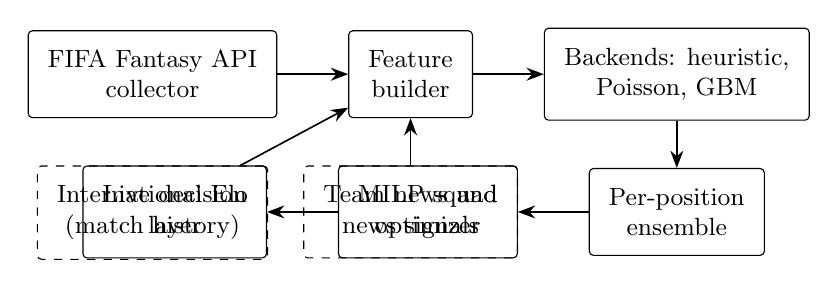
\begin{tikzpicture}[
      node distance=6mm and 9mm,
      box/.style={draw, rounded corners=1.5pt, align=center,
                  minimum height=8mm, inner sep=2.5mm, font=\small},
      ext/.style={box, dashed},
      arr/.style={-{Stealth[length=2.2mm]}, semithick},
    ]
    \node[box] (collector) {FIFA Fantasy API\\collector};
    \node[box, right=of collector] (features) {Feature\\builder};
    \node[box, right=of features] (models) {Backends: heuristic,\\Poisson, GBM};
    \node[box, below=of models] (ensemble) {Per-position\\ensemble};
    \node[box, left=of ensemble] (optimizer) {MILP squad\\optimizer};
    \node[box, left=of optimizer] (live) {Live decision\\layer};
    \node[ext, below=of collector] (elo) {International Elo\\(match history)};
    \node[ext, below=of features] (news) {Team news and\\news signals};
    \draw[arr] (collector) -- (features);
    \draw[arr] (features) -- (models);
    \draw[arr] (models) -- (ensemble);
    \draw[arr] (ensemble) -- (optimizer);
    \draw[arr] (optimizer) -- (live);
    \draw[arr] (elo) -- (features);
    \draw[arr] (news) -- (features);
  \end{tikzpicture}
  \caption{System architecture: data collection, feature construction,
    the three prediction backends and their ensemble, squad
    optimization, and the live decision layer. Dashed boxes are
    external signal sources.}
  \label{fig:architecture}
\end{figure}

\subsection{Pipeline architecture}
\label{sec:implementation-pipeline}

The pipeline is a linear chain of stages mediated entirely by files
on disk. The collector snapshots the three FIFA Fantasy endpoints
into raw Parquet tables; the external module fetches international
match history and club-level CSVs and derives the country and club
Elo tables; the feature builder joins these into a per-player,
per-round feature table; each model backend reads that table and
writes a predictions table; the optimizer reads predictions and
writes a recommendation as JSON and Markdown; and a report generator
renders static HTML from the accumulated JSON. Because every stage
reads from and writes to disk, the pipeline is idempotent: any stage
can be re-run with different parameters without re-running its
upstream stages, and only the collector and external fetchers touch
the network at refresh time.

The repository mirrors this dataflow. The Python package under
\texttt{src/fifa\_fantasy/} holds one subpackage per stage
(\texttt{collector}, \texttt{external}, \texttt{features},
\texttt{model}, \texttt{optimizer}, \texttt{live}, \texttt{web}),
plus a single canonical scoring module shared by training,
validation, and reporting. Data directories separate raw collector
snapshots, derived external tables, processed feature and prediction
tables, training dumps, and per-run recommendation outputs; the test
suite and ad-hoc analysis scripts live alongside. Model artefacts
are stored in LightGBM's text format so they diff cleanly under
version control.

\subsection{Engineering decisions}
\label{sec:implementation-engineering}

Four decisions deserve explicit mention.

\paragraph{Parquet as the interchange format.}
Every intermediate table is Parquet rather than CSV: typed columns,
smaller files, and faster reads across the many re-runs a live
tournament demands. The only hand-maintained CSV is the static FIFA
ranking snapshot of Section~\ref{sec:data-rankings}.

\paragraph{Self-documenting result files.}
Every recommendation file is named with the originating hostname,
backend, stage, and a UTC timestamp. This prevents two collaborators
from clobbering each other's runs and makes the results directory an
audit trail: the JSON carries the full squad with per-player
metadata, lineup and captain decisions, transfer blocks, and
quantile bands where the GBM backend supplies them.

\paragraph{Deterministic training.}
All LightGBM \citep{ke2017lightgbm} training runs pin the seed, the
bagging and feature-fraction seeds, and the library's deterministic
flag. Without this, held-out RMSE wobbles from run to run by enough
to mask small feature-ablation effects; determinism was a
precondition for the A/B comparisons of
Section~\ref{sec:negative-results}.

\paragraph{Exact optimization over greedy selection.}
Squad selection under a budget cap, per-country limits, position
quotas, and a transfer quota has too many interacting constraints
for a greedy heuristic to be trustworthy. We formulate it as a
binary integer program in PuLP \citep{pulp} and solve with CBC
\citep{cbc}; the instance solves in under a second on commodity
hardware, so exactness costs nothing operationally.

\subsection{Reproducibility}
\label{sec:implementation-reproducibility}

Every direct dependency is pinned to a known-good version, model
training is deterministic given the seed, and Monte Carlo
simulations use a fixed NumPy generator seed. The static inputs (the
ranking snapshot, the cached match-history CSV, the club-level CSVs)
are committed to the repository or cached under a versioned
directory, and the pre-tournament FIFA Fantasy snapshot is committed
as well, so a fresh clone reproduces the full pipeline end-to-end
without any network access.

\subsection{Testing}
\label{sec:implementation-testing}

The pytest suite comprises \TestCount{} tests at the pre-final
freeze. The largest share pins the scoring functions:
parametrised cases cover every per-position scoring component
(appearance, goals, assists, clean sheets, conceded-goal penalties,
save bonuses, and the ownership-threshold conditions of the scouting
bonus), together with realistic end-to-end scenarios pinned to known
point totals. The collector, feature builder, and optimizer each
have dedicated test modules backed by end-to-end pipeline runs.
Model correctness is guarded by the held-out validation on the
English Premier League data of Section~\ref{sec:data-fpl}
\citep{vaastav}: any backend change that drifts held-out RMSE by
more than 0.05 in either direction is caught when the validation is
re-run.

\subsection{Team-news ingestion}
\label{sec:implementation-team-news}

Expert fantasy practitioners read manager press conferences roughly
24 hours before kickoff to anticipate rotation, suspensions, and
lineup changes. Our pipeline initially had no such input, so we
built a team-news subsystem that converts published pre-match
previews into a per-fixture predicted-XI signal.

\paragraph{The predicted-XI signal.}
Per-source parsers extract raw lineups (player names as printed,
with a starting or bench status) from public previews and persist
them as one row per fixture, player, and status. The feature builder
joins the most recent lineup per fixture into the feature table as
two columns: a three-valued starting indicator (confirmed start,
confirmed bench, or missing when no news exists) and a confidence
score in $[0,1]$ inherited from the source. The join is NaN-safe by
construction: with no news, both columns are missing and every
backend behaves exactly as before, which we verified by re-running
the backtest with the wiring in place and no data (all backend
totals were unchanged).

\paragraph{Name matching.}
Scraped names must be resolved to FIFA player identifiers. The
matcher normalises case and strips accents, then applies tiered
rules with descending confidence: an exact full-name match (1.00), a
match on the display name such as a mononym (0.95), a last-name
match within the player's country and position (0.85), within the
country alone (0.70), and a last-name match with no country context
(0.50). Ambiguous candidates at any tier abort the match rather than
guess, and unmatched names are logged for manual review; multi-part
Latin American and African naming conventions are the main source of
false negatives.

\paragraph{Availability discount.}
The lineup signal feeds availability handling in two ways. First, a
hard gate: the deterministic backends zero the prediction of any
player with a confirmed bench status, exactly as they do for
transferred or eliminated players, while the Monte Carlo backend
scales simulated points by the confidence score instead of zeroing,
damping low-confidence reports. Second, a soft participation
discount applied to effective points just before optimization: each
player's recent participation rate (the share of their team's
completed matches in which they took the pitch) maps linearly to a
multiplier between a floor of 0.5 and 1. The floor is deliberately
non-zero because participation is measured by a scored-points proxy,
so a nailed starter who blanked twice would otherwise be
misclassified as a rotation risk. Missing participation history
means factor 1 before the tournament (no claim either way), but once
any player has history, a missing value means the player has never
taken the pitch and is treated as the floor; without this rule the
optimizer favoured cheap third-choice goalkeepers whose team-level
clean-sheet points equalled the starter's.

\paragraph{What actually produced data.}
We implemented three source paths: an integration with a
community-maintained scraping library (scaffolded pending confirmed
World Cup coverage), a parser for ESPN pre-match preview articles
that requires the operator to supply article URLs, and a third-party
predicted-lineup site whose parser was never tuned. In practice only
the manual ESPN path produced predicted-XI rows: the scheduled
unattended runs wrote empty snapshots throughout the tournament, so
the signal reached the models only when we hand-fed article URLs
ahead of selected fixtures, with coverage skewed toward high-profile
matches. A companion collector for coarser news signals (headline
and summary feeds filtered by tournament keywords) supplies the
second dashed input of Figure~\ref{fig:architecture}. The scraping
engineering underneath both (client fingerprinting, caching, rate
limiting, retries) is deliberately generic and separated from the
fantasy-specific parsers; we document it in the repository rather
than here.

\section{Validation}
\label{sec:validation}

\subsection{Validation strategy}
\label{sec:validation-strategy}

No World Cup data exists before the tournament starts, so we validate
on the closest available proxy: the English Premier League fantasy
game, whose scoring rules are nearly identical to those of the FIFA
World Cup Fantasy game (the two games share a common heritage). A
model that ranks players well on EPL data should rank players well on
tournament data, subject to the distribution-shift caveats analysed
in Section~\ref{sec:analysis}.

We hold out gameweeks 30--38 of the 2024--25 season (the last nine
gameweeks) and train on all earlier rows of the three-season corpus
of Section~\ref{sec:data-fpl} (2022--23, 2023--24, and 2024--25
through gameweek 29). Held-out error is the per-position root mean
squared error (RMSE) between the predicted score and the realised
\texttt{total\_points}. All three backends of
Section~\ref{sec:methodology} score exactly the same held-out rows,
so the comparison is paired; the per-position row counts appear in
Table~\ref{tab:holdout-rmse}.

\subsection{Held-out results and backend routing}
\label{sec:validation-holdout}

Table~\ref{tab:holdout-rmse} and Figure~\ref{fig:holdout-rmse} report
the held-out RMSE. No single backend wins everywhere; the winners
split cleanly by position.

\begin{itemize}
\item \textbf{Goalkeepers: Poisson} (\RmseGkPoisson{} against
  \RmseGkGbm{} for the GBM). Goalkeeper scoring is dominated by
  appearance and clean-sheet points, and the clean-sheet probability
  is exact under the Poisson goal model, so the structural backend
  captures most of the available signal directly.
\item \textbf{Defenders: heuristic} (\RmseDefHeuristic{}). The
  price-coefficient-times-matchup formula tracks defender outcomes
  better than the GBM at this data scale.
\item \textbf{Midfielders and forwards: GBM} (\RmseMidGbm{} and
  \RmseFwdGbm{}). Individual variance is largest at the attacking
  positions, and the GBM has room to learn non-linear interactions
  that a compact hand-written formula cannot capture.
\end{itemize}

This routing is not merely descriptive: it defines the per-position
ensemble backend, which runs the component models and keeps, for
each position, the prediction of the routed winner. A sixth candidate
GBM feature, the team Elo difference, was evaluated under the same
protocol and rejected; we report that negative result in
Section~\ref{sec:negative-results}.

\subsection{Two GBM iterations}
\label{sec:validation-gbm}

The GBM column of Table~\ref{tab:holdout-rmse} is the second
iteration of the model. The first (v1) trained on a single EPL season
with LightGBM defaults, 31 leaves and 400 boosting rounds
\citep{ke2017lightgbm}; the second (v2) trains on all three seasons
with a lighter sweep-tuned configuration, 15 leaves and 200 rounds,
and improves the held-out RMSE at every position. The defect that
motivated the sweep was visible in squad space before it was visible
in aggregate error: v1 squads were aggressive and implausible, with
clusters of cheap defenders from unfancied squads promoted by a
handful of training rows, a classic signature of too many leaves on
too little data. The v2 squads are conventional. We treat this as a
practical reminder that inspecting the downstream decisions catches
failure modes that aggregate metrics dilute.

\subsection{Determinism and the noise floor}
\label{sec:validation-determinism}

Feature evaluation at these effect sizes requires reproducible
training. Before we pinned the random state, identical code on
identical data produced per-position RMSE values that varied by
roughly $\pm 0.05$ between runs, driven by LightGBM's bagging
randomness. That wobble was large enough to mask the Elo-feature
comparison above: the first attempt produced mixed deltas
indistinguishable from noise. Setting \texttt{seed},
\texttt{bagging\_seed}, \texttt{feature\_fraction\_seed}, and the
deterministic flag collapsed the run-to-run variance to zero and made
the comparison honest. We now treat the pinned seed as part of the
training contract: every RMSE reported in this section is exactly
reproducible.

\subsection{Leak-free walk-forward validation on tournament data}
\label{sec:validation-walkforward}

The EPL hold-out cannot detect EPL-to-tournament distribution shift,
and it cannot evaluate features that only exist once tournament
rounds complete. Mid-tournament we therefore added a second protocol:
leak-free walk-forward validation on realised World Cup rounds. For
each completed round $k \ge 2$, the GBM trains on all EPL rows plus
the WC rounds strictly before $k$, then predicts round $k$; round 1
is excluded because no prior tournament round exists from which to
compute form. Squared errors are pooled across held-out rounds 2--6
to give the per-position and overall RMSE of
Table~\ref{tab:walkforward}; Figure~\ref{fig:walkforward} shows the
per-round traces. Six configurations are compared; the last two draw
on a community-maintained dataset of real match statistics
\citep{mominul2026dataset} that became part of the pipeline before
the final round.

\begin{itemize}
\item \textbf{A: EPL only, no form.} The shipped v2 model: five price
  and team-strength features, trained on EPL rows only. This
  configuration is form-blind; no feature tells it how a player has
  actually performed in the tournament.
\item \textbf{B: EPL only, plus form.} Adds \texttt{form\_lag}, the
  trailing mean of the player's realised fantasy points over the
  previous three matches, shifted by one match so a row's label never
  enters its own feature. One definition is shared by EPL training,
  WC label extraction, and WC inference; a player's first match
  yields a missing value, which LightGBM handles natively.
\item \textbf{C: EPL plus WC, plus form.} As B, but the training set
  also includes every realised WC round before the held-out round,
  recalibrating the output scale to the tournament.
\item \textbf{D: EPL plus WC, proxy minutes.} As C, plus a lagged
  start-rate feature (participation proxied by positive scores) and a
  team goals-conceded form feature.
\item \textbf{E: EPL plus WC, real xG form.} As C, plus the trailing
  mean of the team's real expected goals for and against over its
  previous three matches, computed leak-free from the community match
  dataset. The columns exist only for tournament rows; EPL training
  rows carry missing values, which LightGBM handles natively.
\item \textbf{F: EPL plus WC, real minutes.} As C, plus real lagged
  start rates and minutes shares from the same dataset's lineup
  sheets, testing whether the failure of configuration D was the
  proxy or the signal.
\end{itemize}

The pooled ordering is unambiguous. RMSE falls from
\WalkforwardPooledA{} (A) to \WalkforwardPooledB{} (B) to
\WalkforwardPooledC{} (C), improving at every position at each step,
with the largest single gain at goalkeeper once tournament labels
enter the training set. Configuration D edges C at goalkeeper and
defender but is worse at midfielder and forward and pools slightly
worse (\WalkforwardPooledD{}). Configuration E improves on C at
\emph{every} position and wins the pool at \WalkforwardPooledE{},
the only feature candidate of the tournament to do so; it was
deployed as the fourth-generation model two days before the final
under a pre-registered rule (deploy only on a pooled improvement of
at least $0.01$ with no more than one position regressing).
Configuration F cleared the pooled threshold only marginally
(\WalkforwardPooledF{}), regressed forwards, and lost to E in the
same run, so real minutes stayed out of the model; we return to it
in Section~\ref{sec:negative-results}. On the round-of-16 feature
set the form-retrained model ranks the elite in-form forwards,
including Mbapp\'e, Kane, and Haaland, at the top of its
predictions, where the form-blind model had buried them below
midfielders from strong teams.

The EPL hold-out of Table~\ref{tab:holdout-rmse} is kept at the
version that defined the ensemble routing. Re-run under the deployed
fourth-generation feature set, the GBM improves at every position on
the same held-out rows (goalkeeper \RmseGkGbmVFour{}, defender
\RmseDefGbmVFour{}, midfielder \RmseMidGbmVFour{}, forward
\RmseFwdGbmVFour{}) while leaving the routing unchanged: the Poisson
backend still wins goalkeepers and the heuristic still edges
defenders.

Because these are genuinely out-of-sample tournament rounds, we take
Table~\ref{tab:walkforward} as the leak-free evidence for the
form-retrained model. The squad-level backend comparison of
Section~\ref{sec:live-results} is partly in-sample for the retrained
GBM and the ensemble, since the deployed model has seen the labels of
the rounds scored there; those columns are upper bounds, not
out-of-sample estimates.

\subsection{What the validation does not measure}
\label{sec:validation-limits}

Held-out EPL RMSE is a useful proxy for prediction quality, but
several phenomena specific to international tournament play are
invisible to it.

\begin{itemize}
\item \textbf{Star international players are absent from training.}
  Messi, Mbapp\'e, Modri\'c, Neymar, and others never appear in the
  EPL feature set, so the EPL-trained GBM scores them on price alone
  and undervalues them systematically. The walk-forward retrain above
  mitigates this once realised tournament rounds accumulate.
\item \textbf{Manager rotation behaviour differs.} EPL coaches rotate
  on fixture congestion; international coaches rotate on group-stage
  clinching. The model has no signal for either.
\item \textbf{Knockout-stage variance is higher.} Single-leg
  elimination games carry different team incentives than round-robin
  group games, and every EPL training row comes from a 38-game
  round-robin schedule.
\end{itemize}

These effects surface in the live-tournament results
(Section~\ref{sec:live-results}) and in the analysis
(Section~\ref{sec:analysis}), not in the held-out RMSE.

\begin{table}[t]
  \centering
  % GENERATED by scripts/paper_tables.py -- do not edit
\begin{tabular}{lrrrr}
\toprule
Position & $n$ & Heuristic & Poisson & GBM \\
\midrule
GK & 180 & 2.698 & \textbf{2.491} & 2.650 \\
DEF & 910 & \textbf{3.141} & 3.400 & 3.187 \\
MID & 1228 & 2.874 & 4.371 & \textbf{2.767} \\
FWD & 368 & 3.515 & 4.560 & \textbf{3.153} \\
\bottomrule
\end{tabular}

  \caption{Held-out EPL RMSE per position and backend. Bold marks the
    per-position winner; this routing defines the ensemble.
    \figsource{fifa\_fantasy.training.validate\_main $\rightarrow$
    data/training/validation\_report.json}}
  \label{tab:holdout-rmse}
\end{table}

\begin{figure}[t]
  \centering
  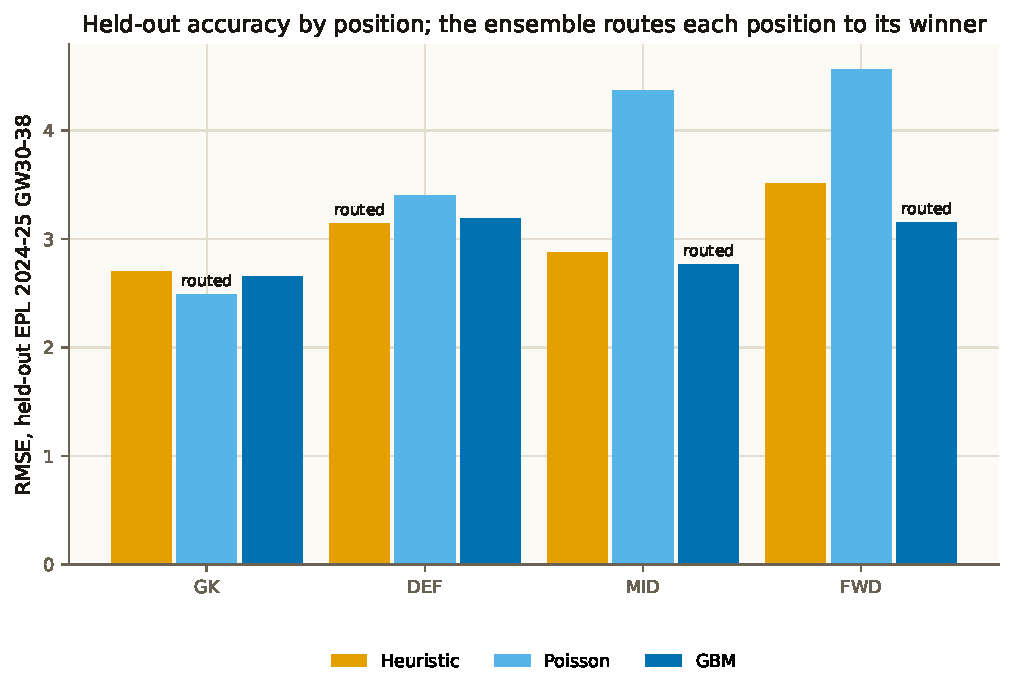
\includegraphics[width=0.85\textwidth]{fig_holdout_rmse.pdf}
  \caption{Held-out RMSE by position and backend.
    \figsource{fifa\_fantasy.report.figures $\rightarrow$
    data/training/validation\_report.json}}
  \label{fig:holdout-rmse}
\end{figure}

\begin{table}[t]
  \centering
  % GENERATED by scripts/paper_tables.py -- do not edit
\begin{tabular}{lrrrrr}
\toprule
Config & GK & DEF & MID & FWD & All \\
\midrule
A: EPL, no form & 3.517 & 3.122 & 3.063 & 3.185 & 3.164 \\
B: EPL + form & 3.350 & 2.962 & 2.776 & 2.984 & 2.952 \\
C: EPL+WC + form & 2.450 & 2.889 & \textbf{2.640} & \textbf{2.757} & \textbf{2.724} \\
D: EPL+WC, all features & \textbf{2.445} & \textbf{2.877} & 2.659 & 2.800 & 2.735 \\
\bottomrule
\end{tabular}

  \caption{Leak-free walk-forward RMSE on WC rounds 2--6, pooled per
    feature configuration. Bold marks the per-column best.
    \figsource{scripts/wc\_forward\_validation.py $\rightarrow$
    data/evaluation/wc\_forward\_validation.json}}
  \label{tab:walkforward}
\end{table}

\begin{figure}[t]
  \centering
  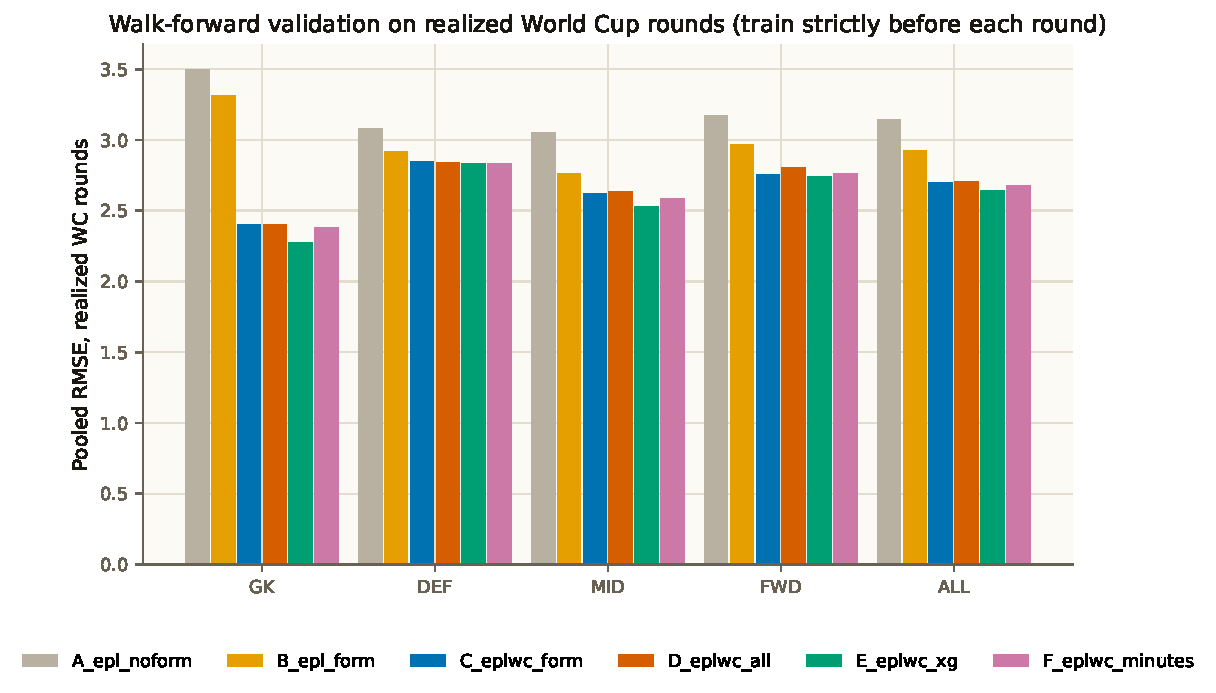
\includegraphics[width=0.85\textwidth]{fig_walkforward.pdf}
  \caption{Walk-forward RMSE per round and configuration.
    \figsource{scripts/wc\_forward\_validation.py}}
  \label{fig:walkforward}
\end{figure}

\section{Live Tournament Results}
\label{sec:live-results}

This section reports how the system performed in live deployment
during the 2026 World Cup. We interleave two records. The first is a
decision log of our actual fantasy entry: for each round we state the
recommendation produced by the models, the decision finally made, the
realised score, and a short post-hoc diagnosis. The second is a
retrospective cross-model backtest that replays every backend
end-to-end on frozen pre-round data, separating the question of how
each backend performs as an autonomous system from how the deployed
entry, which mixed model recommendations with domain judgement,
performed. Table~\ref{tab:backtest-rounds} gives per-round realised
points for both records, Figures~\ref{fig:backtest-cumulative}
and~\ref{fig:backtest-rounds} plot the cumulative and per-round
trajectories, and Table~\ref{tab:season-summary} tracks the official
(ensemble) recommendation against the actual entry and a random-squad
baseline.

\subsection{Cross-model backtest protocol}
\label{sec:live-protocol}

For each completed round we load the feature snapshot closest in
time to, but strictly before, the round's transfer deadline, run
every backend on that snapshot, and pass each backend's predicted
points to the MILP optimiser of Section~\ref{sec:methodology}, which
selects a 15-player squad and an 11-player starting eleven under the
stage's budget and country-cap constraints. The selected squad is
then scored with realised round points from the latest collector
snapshot. As a floor reference we also draw 1{,}000 budget- and
constraint-valid random squads per round and report the mean of
their realised scores. The replay script ships with the repository
and runs with a fixed random seed.

One caveat governs every comparison in this section: the backtest
grants each backend unlimited free transfers every round, whereas
the live entry is limited to two free transfers per stage
transition, with a three-point penalty per extra transfer. Backend
totals are therefore an upper bound on standalone model performance
rather than a like-for-like comparison with the actual entry, whose
figures are net of all transfer penalties incurred. A
constrained-transfer replay is deferred to
Section~\ref{sec:future_work}.

\subsection{Group stage decision log}
\label{sec:live-group}

\paragraph{Matchday 1: initial squad.}
The pre-tournament squad was assembled from the backends'
recommendations combined with domain priors, with the heuristic
backend as the primary live signal and the Poisson and GBM backends
as cross-checks. The pre-tournament call to include Willian Pacho
(Ecuador, defender, \$4.4M) came from the second author's match
observation; Pacho went on to return 11 points across the group
stage at 5.8\% ownership, one of the squad's best returns per
million. We captained Lautaro Mart\'{\i}nez (Argentina, forward,
\$8.8M, 3.2\% ownership) in a 4-4-2. The round realised 33 points,
last place in our personal league. Three failure modes dominate the
diagnosis. First, the captain blanked: Mart\'{\i}nez returned 1 point,
doubled to 2, and the captaincy multiplier is the largest single
variance source in a round. Second, a France triple-stack (Dou\'e,
Olise, and Demb\'el\'e at \$7.5M, \$9.5M, and \$10.0M) shared output
rather than concentrating it, returning 12 points across three
premium midfield slots. Third, none of the four defenders kept a
clean sheet, and Argentina's clean sheet went unexploited because no
Argentine defender was paired with Emiliano Mart\'{\i}nez in goal.

\paragraph{Matchday 2.}
With two free transfers available, the optimiser's best two-transfer
move was to sell Olise and Pacho for Saka and Iba\~nez. We rejected
the Olise sale on domain grounds: Olise had been the squad's top
Matchday~1 scorer with 6 points and plays for a tournament
favourite. The deciding input was the second author's read on
Olise's form, and the captaincy was moved from Mart\'{\i}nez, who was
transferred out, to Olise. The round realised 84 points net, the
entry's largest group-stage total. Olise returned 9 raw points,
doubled to 18 as captain, the squad's largest captain return of the
group stage; Demb\'el\'e's 12 points justified retaining the
remaining France pair; Gakpo added 19; and James and Pacho
contributed 9 each in defence. (An earlier internal draft recorded
this round as 102 points; the realised total in the scoring artifact
is 84, and we report realised figures throughout.) The post-hoc
reading is symmetric: the optimiser was right that Olise carried
future ceiling, and the domain override was right that selling him
was wrong. For a premium player in form, anchoring on form beat the
model's expected value by roughly the margin the captaincy
multiplier implies.

\paragraph{Matchday 3.}
Both free transfers were used and two additional paid transfers were
taken at a cost of six points, bringing in Daniel Mu\~noz, Alexander
Freeman, Ronald Ara\'ujo, and Deniz Undav while keeping Messi as
captain in a 5-2-3. The central risk in the final group round is
rotation, since teams that have already clinched their group rest
starters. The rotation-risk flags for this round, including which
clinched teams would rotate, again came from the second author's
reading of observed squad management; the model carried only a
country-level multiplier and proved too conservative. Selling Pacho
ahead of Ecuador's fixture against Mexico was correct in spirit:
Mexico won and Pacho's defensive return was modest. The round
realised 46 points gross and 40 net of the transfer penalty (the
in-app display showed 42; we note the two-point reconciliation for
completeness and report the artifact figure). Captain Messi returned
7 raw points, doubled to 14, against Jordan: a defensible pick,
although in retrospect Demb\'el\'e outscored him within the same
starting eleven. The paid transfers returned roughly the six points
they cost, a net-zero outcome consistent with the unforced-hit cost
discussed in Section~\ref{sec:lessons}.

\subsection{Knockout rounds}
\label{sec:live-knockout}

\paragraph{Round of 32: wildcard rebuild.}
We played the wildcard, which permits unlimited transfers without
penalty, and rebuilt the squad almost from scratch from the
post-group candidate pool: Rangel and Beach in goal; Laporte,
Cucurella, Mu\~noz, Nuno Mendes, and Freeman in defence;
Demb\'el\'e, Vin\'{\i}cius, Bellingham, Olise, and Manzambi in
midfield; Messi, Haaland, and Undav up front. Total cost was
\$102.9M against the \$105.0M knockout-stage cap. The optimiser
marginally preferred Messi as captain; we chose Demb\'el\'e on
differential grounds, at 19.7\% ownership against Messi's 37.8\%.
The realised outcome of the round appears in
Table~\ref{tab:backtest-rounds}.

\paragraph{Round of 16 and quarter-final.}
The entry scored 66 points net in the Round of 16 and 73 in the
quarter-final, in-app records taken as primary (the squad sheets for
these two rounds were not archived in the repository, an operational
lapse we note for completeness; every other round's squad is
registered pre-deadline). Both rounds continued the wildcard squad's
France--Spain--England spine under the four-transfer knockout quotas.
The quarter-final was the entry's second-best round of the
tournament and beat every backend replay except the GBM's 76
(Table~\ref{tab:backtest-rounds}): the ensemble replay managed 64,
the random baseline 22.5.

\paragraph{Semi-final.}
The semi-final decision is the best-documented of the tournament
because it was registered as a pre-round head-to-head against the
model (the artifact behind Section~\ref{sec:analysis}'s override
analysis). Entering the round with two free transfers and \$1.0M in
the bank, the optimiser's remaining recommendation was to sell
Mac~Allister for Dou\'e and a dead bench slot for Spence; the
operator declined both and kept the squad. The captaincy went to
Mbapp\'e (vice Messi) with the Clean Sheet Shield booster active,
and the pre-round simulation put the operator's pick within one
expected point of the model's (59.7 versus 60.5). The round realised
37 points net, the worst of the knockouts: France lost the
semi-final 0--2 to Spain and the entry's France triple stack
returned four raw points between Maignan, Upamecano, Demb\'el\'e,
and the captain, whose doubled score was 2. The two Spain defenders
(Laporte 7, Cucurella 6) and Messi's 8 kept the round from single
digits, and the Shield converted Argentina's single goal conceded
into one extra point for Mac~Allister, reconciling the recorded 37
with the 36 an id-based rescore produces. The backend replays fared
little better (ensemble 37, GBM 59); with only two fixtures, a
semi-final round's realized total carries high variance under any
selection policy. After the semi-finals the entry stood
at \GlobalRankSF{} in the global game, on 418 points net across the
seven completed rounds.
\paragraph{Final round.}
Round 8 covered both closing matches (the third-place match and the
final), and the deadline was the bronze kickoff, so the round was
planned as a whole. The locked plan moved five transfers into the
eventual champion's block, where Sim\'on, Porro, Cubars\'i, and
Baena joined Laporte and Cucurella for six Spain starters, with the
Qualification Booster active and Mbapp\'e captaining the bronze
match. One further slot went to a second England midfielder as
bronze-game cover, a buy the model rated below its Spain
alternatives and that returned nothing. A planned mid-round armband switch to Messi had to be
abandoned when live play established that the app locks the
captaincy at the captain's own kickoff, contrary to the help-page
wording (the rules transcription and the live tooling have been
corrected accordingly); the operator therefore committed a static
5--3--2 before the bronze kickoff, benching Kane on a rotation read
and starting a fifth defender. Both calls at the operator's
discretion were correct: Kane never played, and the model's one
clear error was the omission of Olise (10 points, started and
scored) from the model-guided eleven. The forecaster's record on
the two matches was one correct call and one miss: the final
matched the modal forecast outcome (Spain 1--0, forecast 54\%),
while the bronze ended England 6--4 over
the 59\%-favoured France, the highest-scoring match of the
tournament and a forecast miss, though Mbapp\'e's hat-trick within
the loss returned 17 raw points, doubled to 34 as captain, the
entry's largest single return of the tournament. The round realised \FinalRoundNet{} points net,
the entry's highest of the eight rounds: the six Spain starters
returned the clean sheet plus the booster's twelve points, and the
season closed at \TotalUserActualNet{} net points and global rank
\GlobalRankFinal{}, an improvement of approximately 250{,}000
places from \GlobalRankSF{} after the semi-finals.

\subsection{Cross-model findings}
\label{sec:live-findings}

Across the seven completed rounds (Table~\ref{tab:backtest-rounds}
and Figure~\ref{fig:backtest-cumulative}), the GBM backend leads the
cumulative leaderboard with \TotalGbm{} points, followed by the
per-position ensemble with \TotalEnsemble{}. Heuristic~v2
(\TotalHeuristicVTwo{}), Monte Carlo (\TotalMonteCarlo{}), and the
original heuristic (\TotalHeuristic{}) form a middle tier, while the
Poisson backend trails the field at \TotalPoisson{}. Every backend
clears the random baseline, whose cumulative mean is
\TotalRandomBaselineMean{} points. Our actual entry stands at
\TotalUserActualNet{} points net of penalties, which is not directly
comparable to the unlimited-transfer backend totals but sits between
the middle tier and the leaders despite paying real transfer costs.
Three observations follow.

First, the Poisson deficit is a genuine mis-calibration finding
rather than noise: the backend systematically over-predicts mean
realised points, and its squads skew toward high-volume,
low-realisation players. We do not recommend deploying it in its
current form, despite its held-out goalkeeper RMSE win
(Section~\ref{sec:validation}), which we now suspect reflects a
small per-position sample; a recalibration pass is queued in
Section~\ref{sec:future_work}.

Second, the captaincy is the highest-leverage single decision in a
round, and it resists prospective optimisation. In each of the three
group rounds the captain that proved optimal within our own starting
eleven was identified only in retrospect: Gakpo over Olise in
Matchday~2 and Demb\'el\'e over Messi in Matchday~3. Per-round
captain outcomes are visible in the round-level spread of
Figure~\ref{fig:backtest-rounds}.

Third, the rounds that went well combined the model signal with
domain judgement (the Olise captaincy, the Pacho pick, the rotation
flags), while the rounds that went poorly weighted one signal over
the other. Table~\ref{tab:season-summary} tracks this round by
round against the official ensemble recommendation.

The closing leaderboard over all eight rounds reads: GBM
\TotalGbm{}, ensemble \TotalEnsemble{}, heuristic~v2
\TotalHeuristicVTwo{}, the actual entry \TotalUserActualNet{} net,
Monte Carlo \TotalMonteCarlo{}, heuristic \TotalHeuristic{}, Poisson
\TotalPoisson{}, random baseline \TotalRandomBaselineMean{}. The
headline comparison is unchanged from mid-tournament but now
complete: the strongest learned backend beats the deployed hybrid
entry under unlimited free transfers, the hybrid entry beats half
the backend field while paying real transfer costs, and everything
beats chance by a factor of three or more. The entry's strongest
rounds (Matchday~2's 84 and the final's \FinalRoundNet{}) were
precisely the rounds where model recommendations and domain
judgement pointed the same way.

\begin{table}[t]
  \centering
  \small
  % GENERATED by scripts/paper_tables.py -- do not edit
\begin{tabular}{lrrrrrrrr}
\toprule
Round & Heuristic & Heuristic v2 & Poisson & GBM & Monte Carlo & Ensemble & User (actual) & Random baseline \\
\midrule
Group Matchday 1 & 46 & 39 & 30 & 105 & 77 & 105 & 33 & 22 \\
Group Matchday 2 & 81 & 79 & 56 & 148 & 79 & 130 & 84 & 23 \\
Group Matchday 3 & 84 & 72 & 44 & 115 & 44 & 94 & 40 & 22 \\
Round of 32 & 73 & 87 & 42 & 108 & 81 & 104 & 83 & 22 \\
Round of 16 & 41 & 63 & 24 & 101 & 56 & 84 & 0 & 20 \\
\midrule
\textbf{Cumulative} & 325 & 340 & 196 & 577 & 337 & 517 & 240 & 105 \\
\bottomrule
\end{tabular}

  \caption{Realized fantasy points per round for every backend replayed
    on frozen pre-round data, alongside the user's actual entry and a
    random-squad baseline.
    \figsource{scripts/model\_backtest.py $\rightarrow$
    data/evaluation/backtest\_summary.json}}
  \label{tab:backtest-rounds}
\end{table}

\begin{figure}[t]
  \centering
  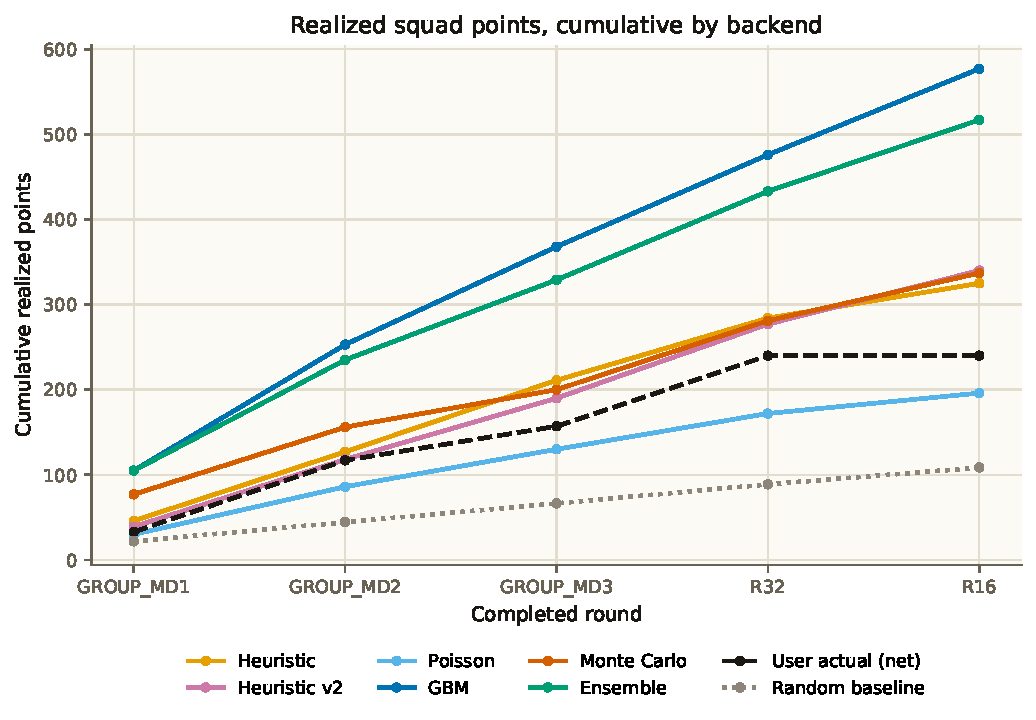
\includegraphics[width=0.85\textwidth]{fig_backtest_cumulative.pdf}
  \caption{Cumulative realized points per backend across the
    tournament.
    \figsource{scripts/model\_backtest.py}}
  \label{fig:backtest-cumulative}
\end{figure}

\begin{figure}[t]
  \centering
  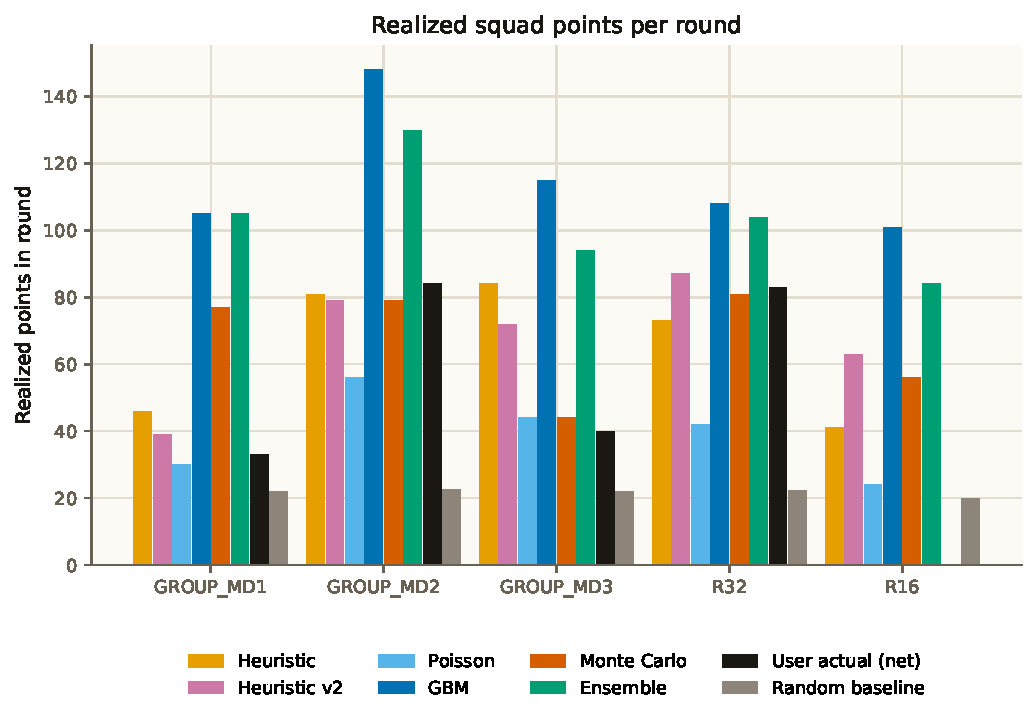
\includegraphics[width=0.85\textwidth]{fig_backtest_rounds.pdf}
  \caption{Per-round realized points per backend.
    \figsource{scripts/model\_backtest.py}}
  \label{fig:backtest-rounds}
\end{figure}

\begin{table}[t]
  \centering
  % GENERATED by scripts/paper_tables.py -- do not edit
\begin{tabular}{lrrr}
\toprule
Round & Ensemble & User (actual) & Random baseline \\
\midrule
Group Matchday 1 & 105 & 33 & 22 \\
Group Matchday 2 & 130 & 84 & 23 \\
Group Matchday 3 & 94 & 40 & 22 \\
Round of 32 & 104 & 83 & 22 \\
Round of 16 & 84 & 0 & 20 \\
Quarter-final & \POSTFINAL{tbd} & \POSTFINAL{tbd} & \POSTFINAL{tbd} \\
Semi-final & \POSTFINAL{tbd} & \POSTFINAL{tbd} & \POSTFINAL{tbd} \\
Final & \POSTFINAL{tbd} & \POSTFINAL{tbd} & \POSTFINAL{tbd} \\
\bottomrule
\end{tabular}

  \caption{Season summary: official (ensemble) recommendation, user
    actual, and random baseline per round.
    \figsource{scripts/model\_backtest.py $\rightarrow$
    data/evaluation/backtest\_summary.json}}
  \label{tab:season-summary}
\end{table}

\section{Analysis}
\label{sec:analysis}

This section examines where the system created value, where it failed,
and what the failures taught us about the structure of the fantasy
scoring problem. Throughout, MD$k$ denotes matchday $k$ of the group
stage and R32 the round of 32.

\subsection{Calibration and sources of value}
\label{sec:analysis-value}

Figure~\ref{fig:calibration} plots pre-match predicted points against
realized points for every scored player-round. Two properties of this
plot frame the rest of the section. First, the predictions carry
genuine rank information: the per-position backend routing selected on
held-out EPL data (Table~\ref{tab:holdout-rmse}) generalized to the
tournament, with the heuristic the safest default for defenders, the
Poisson model for goalkeepers, and the GBM for attacking positions, and
no backend materially contradicted its own player ranking from round to
round. Second, the scale is compressed: realized points span a far
wider range than predicted points. This compression is not a defect of
any single backend but a structural property of mean prediction under
low-count scoring events, and it motivates the variance analysis in
Section~\ref{sec:analysis-variance}.

Beyond point prediction, two components delivered value that is easy to
under-credit. The rolling Elo signal (Section~\ref{sec:data-elo})
corrected real fixture mispricings: when the static FIFA ranking placed
Norway behind Senegal but the post-MD1 rolling Elo ranked Norway ahead,
the heuristic and Poisson backends adjusted Norway players upward by
approximately one expected point. This is the canonical case for
deriving live signals from realized results rather than hand-maintaining
static snapshots.

The MILP optimizer contributed in a way that RMSE cannot measure: it
kept every submitted squad legal. Budget, country-cap, and transfer
quota constraints are non-trivial to satisfy by hand under pre-deadline
time pressure. The solver never produced an illegal squad, and it
surfaced budget infeasibilities immediately (for example, that the
double swap Lautaro Mart\'inez to Messi plus Dou\'e to Bellingham costs
\$2.0M more than the available budget) rather than after a manual
mistake.

\subsection{Failure modes}
\label{sec:analysis-failures}

Three failure modes recurred. The first is GBM blindness to non-EPL
stars. The GBM has zero training rows for Messi and scores him from
price alone, adjusted downward by rotation-conservative status
defaults: at the R32 deadline the heuristic predicted 8.5 points for
Messi while the GBM predicted 2.2. A manager following the GBM alone
would have missed the tournament's top scorer. The heuristic backend,
whose price and matchup terms do capture such players, compensated
within the ensemble, but the premium tier remained the GBM's weakest
segment.

The second is coarse rotation-risk modeling. Our rotation multiplier
was a hand-set per-country scalar (for example 0.55 for Germany at MD3,
after Germany had clinched). A single scalar compresses three distinct
questions: who starts, for how many minutes, and whether the
replacement matters for fantasy purposes. A per-player signal informed
by manager press conferences would have been materially better; no such
feed existed. Section~\ref{sec:analysis-minutes} describes the partial
remedy we shipped.

The third is cross-domain distribution shift. Any feature whose range
at training time differs from its range at inference time is a risk,
and for attacking positions the GBM consistently under-predicted
premium international players relative to their realized totals.
Feature candidates rejected on these grounds are reported in
Section~\ref{sec:negative-results}.

A related operational failure concerns transfer hits. Each transfer
beyond the free quota costs 3 points, roughly 5\% of a typical
group-stage round for our squads, and hits compound. A hit is justified
only when the incoming player is expected to outscore the outgoing one,
net of captaincy implications, by more than 3 points over the planning
horizon. The model's transfer-with-hit logic was systematically too
aggressive because it underestimated rotation: the MD3 hits each cost 3
points and returned roughly 1 in realized output.

\subsection{The goalkeeper paradox}
\label{sec:analysis-gk}

The tournament produced one finding we did not anticipate: the best
real-world goalkeepers were not the best fantasy goalkeepers, and the
model structurally failed to predict this. Through the group stage,
Emiliano (Dibu) Mart\'inez of Argentina, widely regarded as the world's
best goalkeeper, totaled 14 fantasy points over three matches, while
Ra\'ul Rangel of Mexico, a competent domestic-league starter, totaled
21, half as much again. Both teams conceded zero goals across the three
matches.

The gap is entirely a save-bonus effect. The scoring rules award a
goalkeeper 2 points for a 60-minute appearance, 5 for a clean sheet,
1 per three saves, 5 per penalty save, and $-1$ per goal conceded after
the first. The save bonus is therefore increasing in shots faced.
Argentina's defense suppressed opponent shots so effectively that Dibu
made roughly one to two saves per match and rarely reached a save-bonus
threshold; Mexico conceded several attempts on target per match, and
Rangel converted them into save bonuses while keeping the same clean
sheets. The best real-world goalkeeper minimizes goals conceded per
shot faced; the best fantasy goalkeeper faces enough shots to
accumulate save bonuses while still shutting the opponent out. These
are different optimization problems.

Our model could not see the difference. The Poisson backend encoded the
save bonus as a flat constant of 1.0 expected points per start,
implicitly treating save opportunities as exogenous to the fixture. The
heuristic backend has the complementary defect: its matchup factor
inflates predictions with own-team strength for every position, but for
goalkeepers a strong own team reduces save opportunities while
clean-sheet probability for an elite defense is already near its
ceiling. Notably, the optimizer still selected Rangel over Dibu for
R32, at \$3.9M versus \$5.0M, but for the wrong reason: with equal
assumed save bonuses the choice was decided by price, and a different
flat constant could as easily have preferred Dibu. The correct decision
was reached through a model artifact, which is to say, fragilely.

The paradox implies a concrete goalkeeper profile: a team that keeps
clean sheets, a moderate level of opponent attacking threat (enough
shots to earn bonuses, not enough to break the shutout), an established
first-choice role, and a low price that frees budget for attacking
premiums. This explicitly contradicts the naive heuristic of buying the
best real-world goalkeeper. More generally, the scoring rules create
non-monotonic relationships between real-world quality and fantasy
value. We observed the same pattern elsewhere: centre-backs in deep
defensive blocks accumulate defensive counts, wide players in
possession-dominant teams see their credit diffused across long
build-up sequences, and substitute forwards on strong teams are worth
nothing unless they play, although price-based estimates implicitly
assume minutes.

\subsection{Empirically revising the save-bonus term}
\label{sec:analysis-gk-formula}

The fix replaces the flat constant with a term linear in opponent
expected goals: the predicted save bonus is $0.50$ times opponent xG
for the fixture. The multiplier was chosen empirically. We swept
candidate multipliers and measured goalkeeper RMSE on the held-out EPL
set (Figure~\ref{fig:gk-sweep}): the error curve has its minimum at
0.50, is shallow between 0.30 and 0.70, and deteriorates on both sides.
Table~\ref{tab:gk-ab} reports the resulting A/B comparison. Goalkeeper
RMSE improves from \GkRmseVOne{} (v1, flat) to \GkRmseVTwo{} (v2,
tuned) on the EPL holdout, with a larger improvement on realized World
Cup goalkeeper rounds; the other positions are unchanged because the
term applies only to goalkeepers. The revised term also has the correct
limiting behavior: a goalkeeper whose opponent creates nothing earns no
expected save bonus, where v1 awarded a full point.

The revision shipped under a two-gate rule: v2 replaced v1 only because
both the EPL held-out error and the realized World Cup error improved.
One objection deserves a direct answer: tuning a multiplier on held-out
data leaks information into the reported error. We tuned a single
scalar on one data set and validated the choice on an independent one,
and the selection among a handful of candidate values leaks little
relative to the size of the evaluation samples in
Table~\ref{tab:gk-ab}. Methodologically this follows
\citet{benter1994computer}: coefficients on plausible signals are
estimated against outcomes, not assumed. Our own first attempt is the
cautionary counterpart. We initially derived the multiplier
theoretically from shot and save rates; the derivation was internally
consistent and empirically wrong, and we report it with the other
negative results in Section~\ref{sec:negative-results}.

\subsection{Minutes and the availability discount}
\label{sec:analysis-minutes}

A benched player scores at most the appearance floor regardless of form
or matchup, so minutes information dominates any refinement of the
point model. The planned team-news pipeline returned zero predicted
lineup records for the World Cup, so the signal had to come from data
we already held. The World Cup player table exposes one realized total
per completed round; a player who took the pitch banks at least the
appearance points, so participation is proxied by a positive round
score. The feature \texttt{start\_rate\_lag} is the trailing fraction
of a player's last three completed rounds with a positive score; on the
EPL side the same feature uses the true starts flag. Both variants are
shifted by one match and are therefore leak-free. The signal is real:
recently ever-present players scored roughly twice as many points on
average as players who had rarely featured, and blanked far less often
(\POSTFINAL{number: participation-bucket means, blank rates, and the
correlation of start rate with realized points}).

The obvious move, feeding the proxy to the GBM as a feature, made the
model worse. Configuration D of the walk-forward study
(Table~\ref{tab:walkforward}), which adds the participation proxy
together with a team defensive-form feature examined in
Section~\ref{sec:negative-results}, regressed the pooled leak-free RMSE
from \WalkforwardPooledC{} to \WalkforwardPooledD{}. Over four rounds
the proxy is noisy, and it is collinear with lagged form (a benched
player already shows low form), so it adds variance the trees cannot
exploit.

The correct layer is the optimizer, not the model. The shipped
availability discount scales a player's effective predicted points by
$0.5 + 0.5 \cdot \texttt{start\_rate\_lag}$, a contraction toward a
floor of one half rather than zero, because the proxy is imperfect and
a nailed starter can blank twice in a row. Replayed on the heuristic
backend across MD1 to R32, the discount lifted realized squad points
(\POSTFINAL{number: realized squad points with and without the
availability discount, MD1--R32}), and the improvement was stable for
any floor between 0.3 and 0.7. The discount also surfaces an explicit
rotation-risk flag in the human-facing report. The lift is modest, but
for an entry at the bottom of its league every point counts.

\subsection{Ceiling-aware captaincy}
\label{sec:analysis-captaincy}

Captaincy doubles one player's score and is the single highest-leverage
decision in the game, and it is where model and manager disagreed most.
In MD1 both chose Lautaro Mart\'inez, who returned one raw point:
agreement, wrong outcome. In MD2 the model preferred Mbapp\'e; the user
overrode to Olise, who returned 9 raw points, the winning call. In MD3
the model preferred Bellingham; the user captained Messi in a favorable
fixture for 7 raw points. In R32 the model preferred Messi and the user
played Demb\'el\'e as a differential. Where they disagreed and the
outcome is known, the human call won, which we attribute to two inputs
the model does not have: an ownership-aware differential strategy
(maximum expected points is not maximum rank improvement for a trailing
entry) and football-watcher information such as visible form and
midweek fatigue.

Across the completed rounds, no backend selected the round-optimal
captain (Section~\ref{sec:live-results}). The root cause is the
objective: the lineup solver chose the captain as the argmax of mean
predicted points, and mean-argmax is the wrong rule for a trailing
team, which needs the highest ceiling rather than the highest
expectation. The GBM already emits a 90th-percentile (q90) head that
the captain choice ignored. A leak-free per-round backtest (train on
rounds before $k$, predict round $k$, form the eleven by mean) compared
captain rules on raw captain points captured across MD2, MD3, and R32:
the pure-ceiling q90 rule captured roughly twice the points of the
shipped mean rule, with an equal-weight blend in between and a
hindsight oracle far above all three
(\POSTFINAL{number: raw captain points captured by mean-argmax, blend,
q90-argmax, and oracle over MD2--R32}). Doubled by captaincy, the gap
amounts to several realized points per round, in a league being lost by
less.

The shipped selector scores captain candidates by
$(1 - c) \cdot \text{mean} + c \cdot \text{q90}$, where the chase
parameter $c$ is the entry's standings percentile: a leader ($c = 0$)
captains the safe mean, a last-placed entry ($c = 1$) captains the
ceiling. The optimizer now overrides the solver's naive pick with this
selector, defaulting $c = 0.9$ for our position near the bottom. For
point-estimate backends with no q90 head the rule degrades to the mean
and nothing breaks.

\subsection{Scoring variance is the strategy}
\label{sec:analysis-variance}

The user observed an oscillation in round scores: one round in the 40s,
the next in the 80s. The realized starter totals (captain double
excluded) were 32, 75, 39, and 73 across MD1 to R32, so the pattern is
real. It is not, however, a controllable cycle. The decisive evidence
is that MD1 and MD2 used the identical eleven starters and scored 32
and then 75: same players, no transfers, output more than doubled.
Fantasy points are driven by goals and assists, which are low-count
events, and an eleven-player squad naturally swings by tens of points
with selection held constant.

A mean point model is structurally unable to reproduce this. Summing
the heuristic's per-round predictions for the actual starters yields a
nearly flat series whose round-to-round standard deviation is a
fraction of the realized one (\POSTFINAL{number: realized versus
predicted round-total standard deviations}), consistent with the
amplitude compression visible in Figure~\ref{fig:calibration}. A
partially predictable component does exist: realized round totals
correlate positively with the average fixture-strength gap of the
starters and, more strongly, with the model's own per-round squad
prediction (\POSTFINAL{number: correlations of realized round totals
with fixture-strength gap and with the model's per-round prediction}).
The high-scoring rounds were the easier-fixture rounds, and the model
ranked rounds usefully even while understating their amplitude, so the
per-round squad prediction is a usable ex-ante ranker of which upcoming
round will be the high one.

The same lens resolves the mid-tournament observation that a
random-pick rival was outscoring the model-driven entry. A single round
proves little: our 42-point MD3 (net of a transfer hit) sits in the low
tail of the same process that produced a 102-point MD2. The honest
comparison is cumulative. Through R32, the ensemble replay accumulated
\TotalEnsemble{} points and the user's actual entry \TotalUserActualNet{}
net points, against a random-squad baseline mean of
\TotalRandomBaselineMean{} (Table~\ref{tab:season-summary}); the
model-driven process is far ahead of chance while remaining behind a
strong human who reads team news.

For a trailing entry in the knockout rounds, the consequence is the
opposite of smoothing the swing: variance is an asset, because a
low-variance strategy locks in the deficit. Concretely: captain by
ceiling, which the optimizer now does by default at our standings;
time aggression toward the rounds the model ranks as fixture-favorable;
prefer low-ownership differentials in those rounds, since a template
captain who hauls converts no rank gain; and do not spend transfers to
reduce round-to-round variance, because for a chaser the variance is
the only thing that can win it.

\begin{figure}[t]
  \centering
  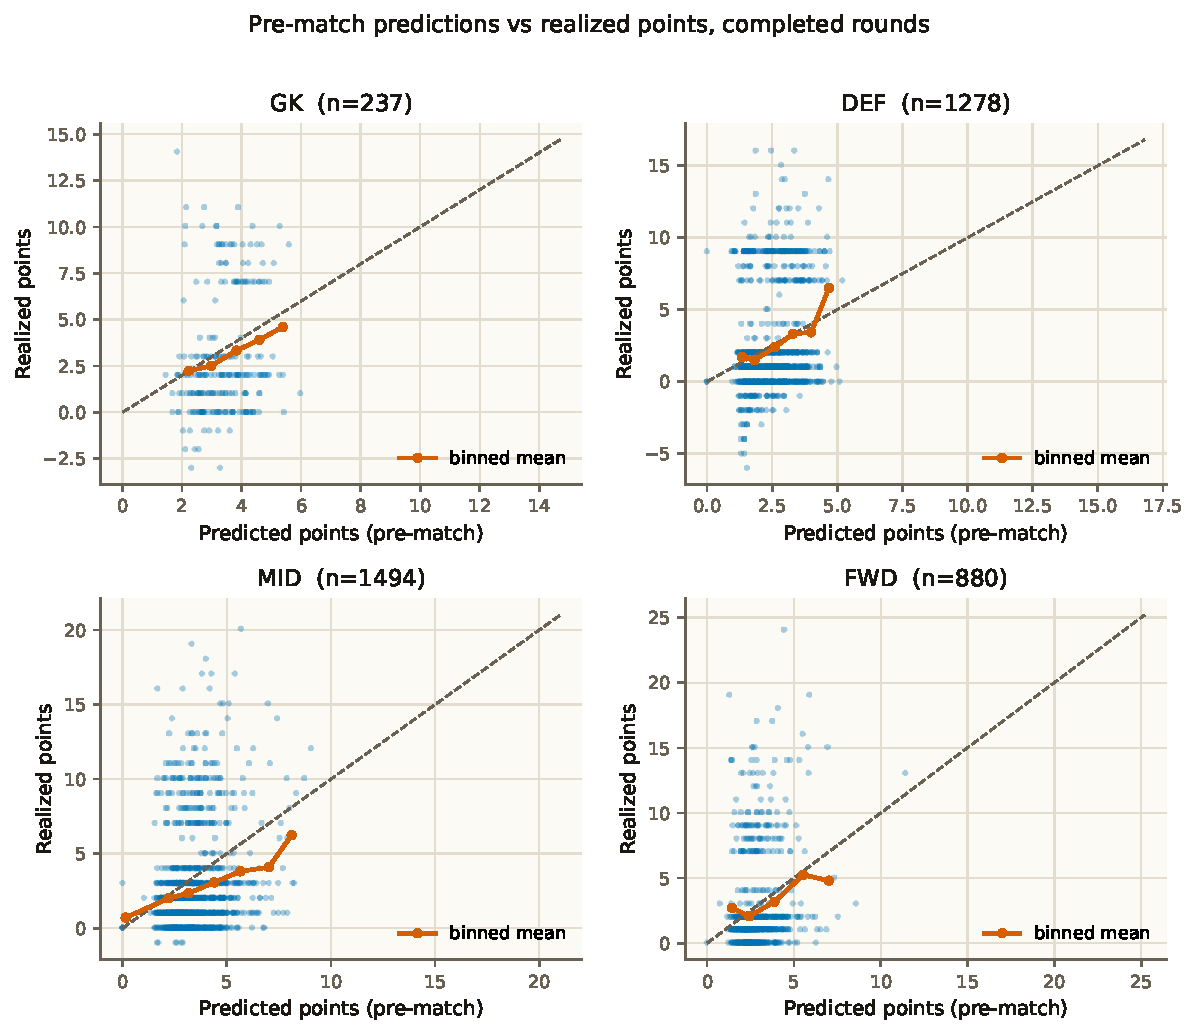
\includegraphics[width=0.85\textwidth]{fig_calibration.pdf}
  \caption{Pre-match predicted points versus realized points.
    \figsource{fifa\_fantasy.report.data.load\_calibration $\rightarrow$
    data/processed}}
  \label{fig:calibration}
\end{figure}

\begin{figure}[t]
  \centering
  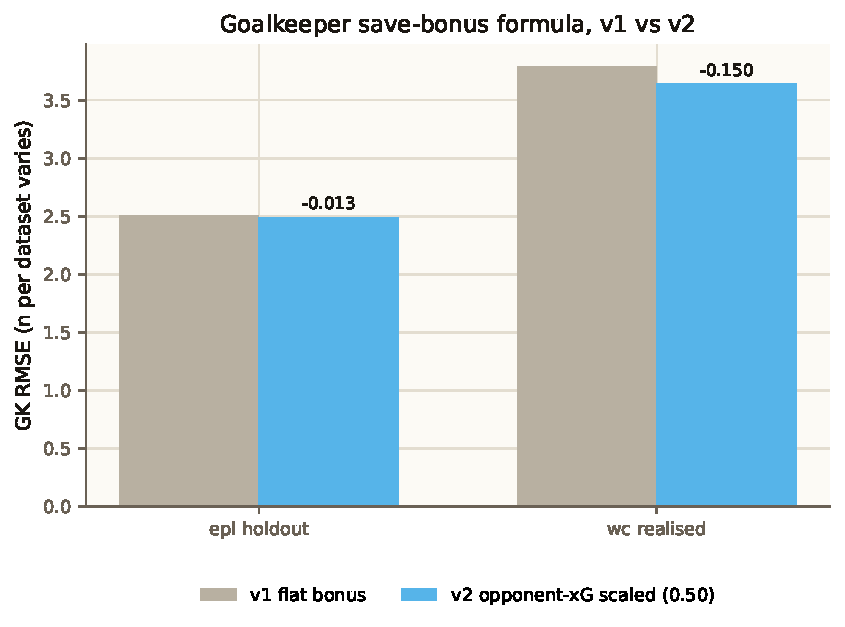
\includegraphics[width=0.85\textwidth]{fig_gk_sweep.pdf}
  \caption{Goalkeeper save-bonus multiplier sweep: empirical RMSE
    across candidate multipliers.
    \figsource{scripts/gk\_formula\_ab.py $\rightarrow$
    data/evaluation/gk\_formula\_ab.json}}
  \label{fig:gk-sweep}
\end{figure}

\begin{table}[t]
  \centering
  % GENERATED by scripts/paper_tables.py -- do not edit
\begin{tabular}{lrrrr}
\toprule
Dataset & $n$ & RMSE v1 & RMSE v2 & $\Delta$RMSE \\
\midrule
epl holdout & 180 & 2.503 & 2.491 & -0.013 \\
epl holdout & 910 & 3.400 & 3.400 & 0.000 \\
epl holdout & 1228 & 4.371 & 4.371 & 0.000 \\
epl holdout & 368 & 4.560 & 4.560 & 0.000 \\
wc realised & 168 & 3.790 & 3.640 & -0.150 \\
\bottomrule
\end{tabular}

  \caption{Goalkeeper save-bonus formula A/B: v1 (flat) versus v2
    (empirically tuned 0.50 multiplier).
    \figsource{scripts/gk\_formula\_ab.py}}
  \label{tab:gk-ab}
\end{table}

\section{Negative Results}
\label{sec:negative-results}

Not every idea we tested survived contact with held-out data. This
section documents six approaches that were implemented, evaluated
under the same gates as every shipped change
(Section~\ref{sec:validation}), and rejected. We report them in full
for two reasons. First, each rejection shaped the production system:
the discipline of adding one component at a time behind a held-out
gate is itself a consequence of the failures below. Second, several
of the hypotheses are natural enough that other practitioners will
try them; the measurements here may save that effort or sharpen it.
Table~\ref{tab:negative-summary} summarizes the six approaches; the
following subsections give one account each. Two failure modes recur:
constants derived from plausible first principles that measurement
contradicts, and signals that are genuinely informative but harmful
when injected at the wrong layer of the system.

\begin{table}[t]
  \centering
  \small
  \begin{tabular}{@{}p{0.26\linewidth}p{0.33\linewidth}p{0.33\linewidth}@{}}
    \toprule
    Approach & Hypothesis & Outcome \\
    \midrule
    Heuristic v2 component stack &
    Six domain-motivated bonuses improve the price-anchored heuristic &
    Trailed unmodified v1 in every backtested group round; reverted \\
    \addlinespace
    \texttt{team\_elo\_diff} as a GBM feature &
    The Elo gap adds fixture signal to the learned model &
    Held-out wash plus distribution-shift risk; signal routed to the
    structural backends instead \\
    \addlinespace
    Theoretical GK save-bonus multiplier (1.13) &
    A first-principles constant prices expected saves correctly &
    Overestimated by roughly a factor of two; empirical sweep
    shipped 0.50 \\
    \addlinespace
    \texttt{start\_rate\_lag} and \texttt{team\_gc\_form} as GBM
    features &
    Participation and team defensive form add predictive signal &
    Regressed leak-free walk-forward RMSE at every position; signals
    rehomed at the optimizer layer \\
    \addlinespace
    Benter combiner with market prices &
    Tournament-winner market probabilities complement model
    predictions &
    Any positive market weight raised RMSE for every backend in every
    round; shipped weight zero \\
    \addlinespace
    GK defensive-form adjustment &
    Recent goals conceded sharpens goalkeeper predictions &
    Worse as a feature and as a Poisson blend; structure beats
    realized form at this sample size \\
    \bottomrule
  \end{tabular}
  \caption{Summary of documented negative results. Each approach was
    implemented and evaluated against held-out or walk-forward data
    before rejection; details and evidence appear in the subsections
    below.}
  \label{tab:negative-summary}
\end{table}

\subsection{Heuristic v2: a six-component stack}
\label{sec:negative-heuristic-v2}

The heuristic backend of Section~\ref{sec:methodology} predicts
points as a position coefficient times price, scaled by matchup and
home factors: three moving parts. A v2 candidate layered six
domain-motivated changes onto it at once: a goalkeeper save bonus
scaled by opponent expected goals; a defender clean-sheet bonus
proportional to $\exp(-\mathrm{xG}_{\mathrm{opp}})$; ball-progression
and goal-conversion bonuses for midfielders and forwards who
outperform their position median; a premium-tier bump for players
priced above \$9.5 million; and a realized-form anchor that blends
the structural prediction toward the player's tournament scoring
average, with a weight growing from zero to 0.40 by four matches
played. Every component was individually defensible, and several
encode genuine features of the scoring rules.

Replayed under the frozen-data backtest protocol of
Section~\ref{sec:live-results}, v2 scored below unmodified v1 in
every completed group round (Table~\ref{tab:backtest-rounds}). Our
diagnosis has four parts. First, the realized-form anchor pulls
toward one to three matches of data, where the per-player average is
dominated by variance; the structural prediction is more reliable
than the realized average at that sample size. Second, the stacked
bonuses shifted squad composition, promoting players (for example,
defenders facing low-xG opponents) who did not in fact outscore the
v1 picks. Third, the premium-tier bump was too small to change the
optimizer's selections and should have been either amplified or
omitted. Fourth, and most generally, six additions give the model six
places to be slightly wrong where v1 has three; on small samples the
misalignments compound rather than cancel.

We reverted to v1 and kept v2 in the repository as a runnable
research backend. We note for completeness that the replay ordering
reversed in later knockout rounds (Table~\ref{tab:backtest-rounds}),
with cumulative totals of \TotalHeuristicVTwo{} for v2 against
\TotalHeuristic{} for v1, which underlines how noisy a three-round
gate is. \POSTFINAL{state whether the v2 knockout-round recovery
persisted over the full tournament and reconcile with the reversion
decision} The procedural lesson stood regardless and became policy:
one component at a time, each behind a held-out gate, with failures
documented rather than discarded.

\subsection{\texttt{team\_elo\_diff} as a GBM feature}
\label{sec:negative-elo-feature}

The gradient-boosted model \citep{ke2017lightgbm} shipped with five
features. A v3 candidate added the Elo gap between a player's team
and the opponent \citep{elo1978rating, hvattum2010using} as a sixth:
club Elo computed from historical match data on the training side,
country Elo aliased to the same column at inference. Under a
deterministic seed, the held-out comparison against v2 was a wash:
small improvements for goalkeepers and midfielders, offset by small
regressions for defenders and forwards, with all four movements
within about one percent.

A wash on its own might still justify shipping, but the feature
carried a structural risk that the aggregate number understates:
distribution shift. Elo gaps between national teams at a World Cup
are several times wider than the club-Elo gaps in the training
league, so the tree ensemble would evaluate many tournament fixtures
in a region of feature space with no training support, where trees
extrapolate by clamping to the nearest leaf. We did not ship v3. The
Elo signal is instead consumed directly by the heuristic and Poisson
backends, where its effect on predictions is monotone by construction
and no extrapolation is involved. A procedural footnote: this A/B was
only legible after we fixed all training seeds, since run-to-run
noise from the boosting procedure's subsampling initially exceeded
the effect being measured.

\subsection{The theoretical goalkeeper save-bonus multiplier}
\label{sec:negative-gk-multiplier}

The Poisson backend's original goalkeeper formula assigned a flat
expected save bonus per start, independent of the fixture. Replacing
the constant with a term scaled by opponent expected goals is clearly
right in direction: the save-bonus rule pays one point per three
saves, and save opportunities are a function of how much attack the
opposing team generates. The question is the multiplier. We first
derived it from football fundamentals: roughly 4.0 shots on target
per unit of opponent xG, a median save percentage of 0.85, and the
one-per-three-saves rule give $4.0 \times 0.85 / 3 \approx 1.13$
expected bonus points per unit of opponent xG.

The derivation was internally consistent and built from three
independently measurable quantities. It was also wrong. On held-out
data the 1.13 multiplier regressed goalkeeper RMSE relative to the
flat baseline it was meant to replace
(Figure~\ref{fig:gk-sweep}). Both inputs were overestimates: much of
opponent xG never becomes an on-target shot, and the median
goalkeeper in the evaluation distribution saves at a substantially
lower rate than the elite keepers who anchor intuition. The two
errors compound multiplicatively. An empirical sweep over candidate
multipliers found its minimum at 0.50, less than half the derived
value, improving goalkeeper RMSE from \GkRmseVOne{} to \GkRmseVTwo{}
(Table~\ref{tab:gk-ab}); the empirical calibration and its A/B
validation are discussed in Section~\ref{sec:analysis}. The lesson we
draw is not that structural derivation is useless (the functional
form survived; only the constant fell) but that a derivation is a
hypothesis, and the sweep, not the algebra, sets the constant.

\subsection{Participation and defensive form as GBM features}
\label{sec:negative-minutes}

A benched player scores at most the appearance floor regardless of
form or matchup, so participation is an obvious candidate signal.
With no reliable predicted-lineup source for the tournament, we
proxied it: \texttt{start\_rate\_lag} is the trailing fraction of a
player's recent completed rounds with a positive score (the true
starts flag is used on the league training side), computed leak-free
with a one-round shift. The signal is real: players with full recent
participation outscore rotation risks by a wide margin and blank far
less often. \texttt{team\_gc\_form}, the trailing mean of goals
conceded by the player's team, was constructed analogously as a
defensive-form signal.

Feeding both to the GBM failed. Configuration D of the walk-forward
validation added the pair to the shipped feature set and regressed
the leak-free pooled RMSE from \WalkforwardPooledC{} to
\WalkforwardPooledD{}, worse at every position
(Table~\ref{tab:walkforward}). Over a handful of tournament rounds
the participation proxy is too noisy, and it is collinear with the
trailing form feature (a benched player already shows low form), so
it adds variance the trees cannot convert into signal; defensive form
is likewise collinear with the strength features the model already
holds. The correct layer turned out to be the optimizer, not the
model: an availability discount scales a player's effective points by
$0.5 + 0.5 \cdot \mathtt{start\_rate\_lag}$ before squad selection,
so the solver stops spending budget on rotation risks. That
adjustment improved realized squad points over the backtested rounds
(\POSTFINAL{number: realized squad points with versus without the
availability discount on the heuristic backend}) and was stable
across a wide band of floor values; it also surfaces a rotation-risk
flag in the operator report. The same walk-forward harness rejected
three further feature-layer candidates in the same review: a
form-times-opponent-strength interaction (within noise), recency
weighting of tournament training rows (monotonically worse for
goalkeepers), and dropping did-not-play rows to match the league
pipeline's minutes filter, which was decisively worse because the
zero-target rows are precisely how the model learns that
low-participation profiles score zero.

\subsection{A Benter-style combiner over prediction-market prices}
\label{sec:negative-market}

\citet{benter1994computer} showed that combining a fundamental model
with market odds can beat either alone, and prediction markets are
efficient aggregators of public information
\citep{wolfers2004prediction}. We therefore tested a combiner that
multiplies each player's model prediction by a country-level
adjustment derived from tournament-winner contract prices on a
prediction market: the most recent pre-deadline implied win
probability per country, normalized by the field mean, entering
through a single free weight $\beta_2$ (intercept and slope fixed at
zero and one). We swept ten values of $\beta_2$ from 0 to 0.30 for
every backend over the completed rounds.

The result was unambiguous. The empirical optimum for every backend
is $\beta_2 = 0$, and RMSE rises monotonically in the market weight.
At the ablation operating point $\beta_2 = \MarketBetaTwo$, enabling
the adjustment worsens RMSE for every backend in every round
(Table~\ref{tab:market-negative}), by \MarketMeanDeltaRmse{} on
average across backends and rounds; Figure~\ref{fig:market-negative}
shows the with-versus-without comparison.

\begin{figure}[t]
  \centering
  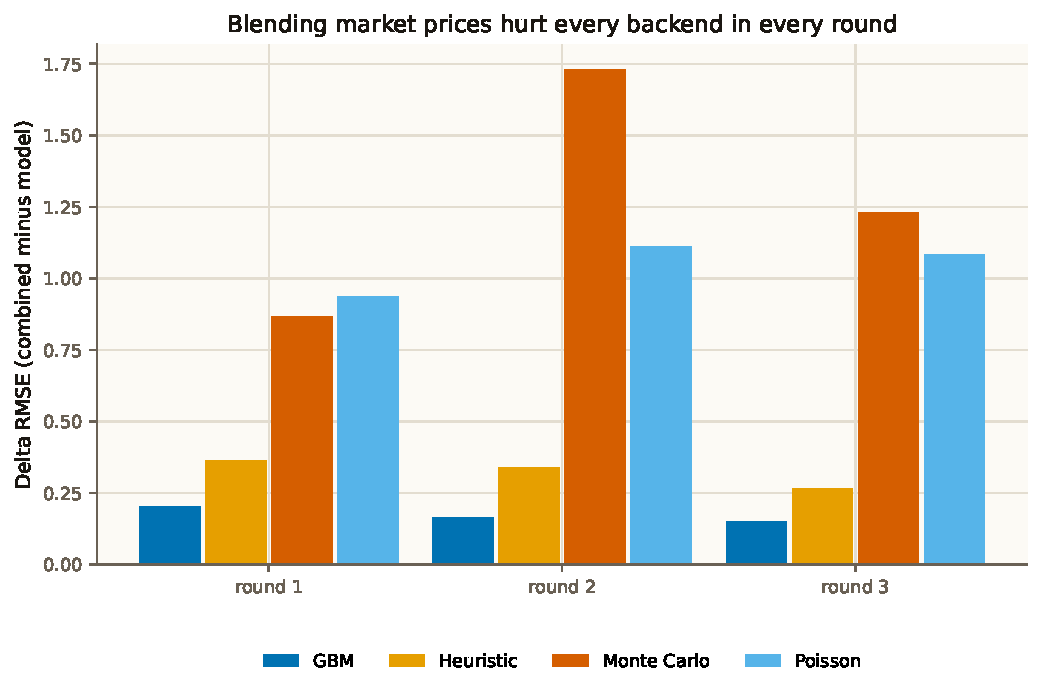
\includegraphics[width=0.85\textwidth]{fig_market_negative.pdf}
  \caption{Effect of blending prediction-market signals into the
    expected-points models: RMSE with versus without the market term.
    \figsource{scripts/with\_vs\_without\_market.py $\rightarrow$
    data/evaluation/with\_vs\_without\_market.json}}
  \label{fig:market-negative}
\end{figure}

\begin{table}[t]
  \centering
  % GENERATED by scripts/paper_tables.py -- do not edit
\begin{tabular}{lrrrr}
\toprule
Backend & R1 & R2 & R3 & Mean \\
\midrule
Heuristic & 0.364 & 0.338 & 0.266 & 0.323 \\
Poisson & 0.938 & 1.111 & 1.084 & 1.044 \\
GBM & 0.201 & 0.163 & 0.150 & 0.171 \\
Monte Carlo & 0.866 & 1.730 & 1.230 & 1.275 \\
\bottomrule
\end{tabular}

  \caption{Per-round change in RMSE ($\Delta$RMSE, positive is worse)
    when the Benter-style market adjustment is enabled
    ($\beta_2 = \MarketBetaTwo$).
    \figsource{scripts/with\_vs\_without\_market.py}}
  \label{tab:market-negative}
\end{table}

We attribute the failure primarily to a granularity mismatch.
Tournament-winner contracts price a season-scale outcome driven by
squad depth, bracket, and long-horizon strength; our target is
per-match, per-player fantasy points, driven by fixture-scale
factors the contract cannot see. What country-level strength the
market does encode is redundant with signals the models already
carry: the implied win probabilities correlate at
\POSTFINAL{number: correlation between market implied win
probabilities and derived country Elo} with our derived country Elo,
making the market term a noisy near-substitute rather than a
complement. Two further effects plausibly contribute: the prices
exhibit the canonical favorite-longshot bias
\citep{thaler1988favorite, snowberg2010explaining}, which our
multiplicative combiner does not correct, and liquidity is
concentrated on a few favorites, so the thin long-shot contracts we
weight symmetrically are dominated by noise. The negative result is
specific to this configuration: tournament-winner contracts at
country granularity, a per-player per-match target, and a
multiplicative combiner. Per-fixture markets at granularities matched
to the prediction target remain untested and are discussed in
Section~\ref{sec:future_work}. We kept the combiner architecture and
the market scraper, shipped a weight of zero (the combiner is a
no-op in production), and demoted market data to descriptive context
on the intelligence page.

\subsection{Goalkeeper defensive-form adjustment}
\label{sec:negative-gk-form}

The last negative result closed the loop on goalkeeper form. Our
working hypothesis was that personal scoring form is noise for
goalkeepers (their points come from clean sheets and saves, not from
repeatable individual scoring) and that the right form signal for the
position is the team's recent defensive record. The first half held
up; the second did not. We tested \texttt{team\_gc\_form} in two
ways: as a GBM feature, where it participated in the configuration D
regression of Section~\ref{sec:negative-minutes}, and blended
directly into the Poisson clean-sheet term, where goalkeeper points
actually originate. Sweeping the blend weight on held-out goalkeeper
rows, RMSE rose monotonically with the weight: the more realized
defensive form we injected, the worse the prediction.

The mechanism is the same one that sinks personal form for the
position. Three or four matches of goals conceded is a tiny,
high-variance sample, and its dominant component is opponent
strength, which the structural model already encodes through the
fixture terms \citep{maher1982modelling, dixon1997modelling}. The
structural Poisson backend remains our best goalkeeper predictor
(Section~\ref{sec:validation}), the ensemble routes goalkeepers to
it, and no defensive-form signal ships. The honest finding is that at
tournament sample sizes no realized-form signal we tested beats
structure for this position, and pretending otherwise would have cost
accuracy. Section~\ref{sec:lessons} generalizes the pattern.

\section{Lessons Learned}
\label{sec:lessons}

This section distils the transferable lessons of building and
operating the system live during the tournament, from the predictive
core, through the decision layer that turns predictions into picks, to
the engineering process around both. Each lesson was learned at the
cost of real ranking points.

\subsection{Realised form must anchor predictions for elite players}
\label{sec:lessons-form-anchor}

Every backend that survived validation was form-blind: it predicted a
player's points from price and relative team strength alone, with no
term for how the player had actually been scoring. The result was our
most consistent failure mode: under-prediction of premium
international stars such as Lionel Messi and Kylian Mbapp\'e, whom the
gradient-boosted model had never seen in its club training data and
therefore compressed toward the price-tier mean while their realised
averages ran far above it. Fed those numbers, the optimiser repeatedly
wanted to bench in-form, ceiling-priced forwards, and we overrode it
by hand. When the operators must routinely ignore the model on the
highest-variance decision in the game, the model is not doing its job.

This was not a data-availability problem: the tournament player table
carried \texttt{round\_points}, realised points per completed round,
from Matchday~1. A trailing form average was computable from day one;
it was simply never computed. The eventual correction needed two parts
working together: a leak-free lagged form feature, and retraining on
realised tournament rounds so the output scale fits the tournament.
The form feature alone, on club-only training, barely moved the
predictions; neither half is sufficient without the other.

\subsection{A designed but undeployed fix scores zero}
\label{sec:lessons-deploy}

Worse, we had anticipated the problem and built the fix, then never
turned it on. The training entry point had an \texttt{--include-wc}
flag, the code that mines realised tournament rounds into training
rows existed, and the README stated the retraining plan in plain
language. That retrain was never run in production: the deployed model
artefacts were last written on June~21 from club data only, and the
snapshot daemon re-scored the player pool every twelve hours for the
entire group stage and round of 32 against that frozen model while
four rounds of realised labels accumulated unused.

Building the retrain path and building the schedule that runs it are
two different tasks, and only the second one scores points. Likewise,
a long-lived process is a deployment target: it must log its code
version at startup and be restarted on deploy, or it will silently run
last month's code against this month's tournament. In one line: build
the loop, validate the loop, and then, separately and deliberately,
run the loop.

\subsection{Rotation risk is a first-class feature, not a fudge
factor}
\label{sec:lessons-rotation}

We modelled rotation risk as hand-set per-country multipliers in a
script: the right intuition at the wrong abstraction level. Rotation
is a per-player decision driven by manager preference, recent minutes
load, and tournament incentives such as an already-clinched group. A
proper treatment would track per-player minutes, score
manager-specific rotation propensity, detect the clinched-group signal
from standings, and output a per-player probability of starting. We
had none of this and paid for it in Matchday~3, where realised
rotation absorbed the expected gain of multiple paid transfers whose
expected-value justification was correct on its inputs. Because a
benched starter scores near zero regardless of form or matchup,
rotation is the largest unmodelled term in the system. The rule we
adopted as a margin of safety: never take an unforced transfer hit
unless the predicted gain over the next two matchdays exceeds twice
the per-hit cost.

\subsection{Captaincy is where human judgment beat the model}
\label{sec:lessons-captaincy}

Across the three group-stage matchdays our manual captain calls beat
the model's recommendation in two of the three rounds; the one loss
was a pick on which the model and the operators agreed. Both wins came
from signals the model did not consume: team news, expected manager
behaviour, and current form. No backend picked the optimal captain in
any group round. The optimiser maximises within-squad mean expected
points, but captaincy doubles a single player and rewards ceiling
rather than mean, as well as ownership differential and
fixture-specific motivation. Captain recommendations should be
advisory rather than prescriptive, and a captain objective should
score the upper quantiles of the predictive distribution, not its
mean.

\subsection{Differential strategy is portfolio construction}
\label{sec:lessons-portfolio}

We initially framed the differential question as a binary choice:
follow the template or chase differentials. The correct framing is
portfolio construction: a mix of template anchors (matching the field
on its likely captain picks, so the rank does not collapse when the
template scores), mid-ownership workhorses that accumulate the bulk of
the points, and low-ownership differential bets that create climb
opportunities when the template blanks, with the mix governed by the
current league standing. Our optimiser maximised raw expected points;
we approximated the portfolio by hand each round. A mean-variance
formulation under the budget and country constraints is the natural
formal treatment (Section~\ref{sec:future_work}).

The tournament also taught us where differentials live. The best
differential returns came from defenders and bench midfielders, while
our one attempt at a premium-forward differential returned nothing
when the player did not start. At the premium forward tier, ownership
is highly correlated with realised production; at the defender and
bench tiers the field under-attends and genuine value persists.
Template at forward, differentiate at defence and on the bench.

\subsection{Goalkeeper save value scales with opponent quality}
\label{sec:lessons-gk}

The Poisson backend priced goalkeeper save points as a flat constant,
assigning the same save expectation to a keeper behind a dominant
defence and one facing sustained pressure every match. Empirically,
expected save points scale with opponent expected goals, strongly
enough to change the goalkeeper ranking. We confirmed this as a model
bug, replaced the constant with a term scaled by opponent expected
goals, and validated the change on held-out data before shipping it
(Section~\ref{sec:negative-results} documents an earlier
mis-calibrated attempt). The general lesson: any component priced as a
constant should be audited for the covariate it silently ignores.

\subsection{Auto-substitution makes the bench an ordered queue}
\label{sec:lessons-bench}

The game's auto-substitution rule replaces a starter who plays zero
minutes with the highest-priority bench player who fits the formation,
so the bench is an ordered queue, not a set of interchangeable
backups. We never modelled the bench-order objective: the optimiser
produced a starting eleven and a bench but no ordering, which we set
by hand every round. Bench order should be a first-class solver
output, ordered by predicted points with the goalkeeper last.

\subsection{Decision-support artefacts should not need a server}
\label{sec:lessons-artefacts}

We initially planned an API service for decision review and pivoted to
a static HTML report. The static report became the highest-utility
artefact of the project: every transfer decision was made by opening
it, reading the captain board, and cross-checking against our domain
priors. The lesson generalises: produce decision artefacts viewable
without infrastructure, with Markdown for permanent records, HTML for
interactive review, and JSON for downstream consumption.

\subsection{The decision layer, not the model, was the weak layer}
\label{sec:lessons-decision-layer}

A structured mid-tournament review found no defect in the model
mathematics that had survived validation, but five distinct bugs in
the layer that turns predictions into picks: an availability discount
whose missing-history policy exempted exactly the never-played players
it existed to catch; the squad and lineup solvers silently optimising
different objective columns; a scouting bonus counted twice on one
backend's path; missing values poisoning the captain sort into
arbitrary order; and a form multiplier whose denominator grew every
round until it pinned all players to its clip floor. These are
plumbing errors, not modelling errors, and unit tests missed them
because every component met its own spec.

What was missing were end-to-end invariants on the artefact users
consume: a never-played player must not start, a captain score must be
finite, a bonus must be counted once, the budget must be within the
cap. Such invariants are cheap and would have caught most of these
bugs at introduction. Relatedly, the meaning of a missing value is a
design decision per column, not a default: three of the five bugs
trace to NaN having no declared meaning.

\subsection{Verify the data contract against a second source}
\label{sec:lessons-data-contract}

The most consequential single finding was in the data. The fantasy API
truncates each player's \texttt{round\_points} list at the last round
in which the player personally recorded anything: interior
non-appearances are zero-filled, trailing ones simply vanish, and
nothing documents this. Every consumer assumed the list length equals
the squad's completed rounds, which was false for
\TruncationShareQf{} of the player pool at the quarter-final
snapshot. The inflation lands exactly on recently-dropped players,
the population the availability discount exists to catch, and it
silently defeated the discount for all of them. The fix reconstructs
the truth from a source the API cannot truncate, the fixture table,
padding \texttt{round\_points} with zeros up to the squad's
completed-fixture count in one function shared by training and
inference. A single assertion comparing list length to completed
fixtures would have caught this in the first week; the cross-check
existed in the data the whole time, and nobody wrote it.

\subsection{Validate one component at a time, and build the harness
first}
\label{sec:lessons-validation-gate}

Twice we shipped theoretically motivated model changes as a bundle and
lost: each addition was individually defensible, and collectively they
degraded performance on every backtested round
(Section~\ref{sec:negative-results}). Simpler models outperform richer
ones on samples this small, because every added component is another
place to be slightly wrong. The decision rule we adopted as binding:
one component at a time; held-out error must improve at the position
of interest before shipping; the live tournament backtest must not
regress for at least one round; and failed attempts are documented,
because honest negatives are results too. The corollary is to build
the walk-forward validation harness first, not in week four: every
modelling decision made before ours existed was evaluated on intuition
or in-sample evidence, and most were later reversed. The harness is
the cheapest component in the repository and the only one that has
never been wrong.

\subsection{Generate every number that appears in the documentation}
\label{sec:lessons-generated-numbers}

A pre-publication audit comparing every claim in the project
documentation against the code found that hand-copied figures had
drifted in 38 places over five weeks: stale feature counts, backend
lists two versions out of date, two sections disagreeing about the
same round's realised score. Every number that was wrong had been
typed by hand; every number that was right was generated by a script
and pasted with its source cited. The lesson is mechanical rather than
moral: documentation numbers must come from script output, with the
generating script cited next to the number, and a drift audit belongs
before publication. This paper practises the rule its drafts violated:
its numeric claims are injected from generated macros rather than
typed.

\section{Future Work}
\label{sec:future_work}

The system was built and operated under tournament time pressure, and
several extensions were deliberately deferred. We collect here the ones
we consider most valuable: richer data sources, upgrades to the score
model and team ratings, principled Bayesian updating, optimizer
extensions, and the prediction-market combiner that we regard as the
main methodological follow-up.

\subsection{Data Sources}
\label{sec:future-data}

The single largest gap during live operation was confirmed starting
elevens. A scraper that monitors manager press conferences, predicted
lineups from major outlets, official team sheets released an hour
before kickoff, and national-team beat reporters, and that emits a
per-player starting probability before each deadline, would have
closed the failure mode that cost us most: rotation by teams that had
already clinched their group.

A source audit conducted during the tournament identified four
additions worth integrating. The \texttt{soccerdata} Python library
wraps eight providers behind one interface and would add shot-level
expected goals, lineups, and historical bookmaker odds useful for
backtest calibration, though its shot-level coverage is limited to
club leagues. The \texttt{worldfootballR} R package is the only
verified route to FBref international coverage, including shot events
and advanced per-match statistics for past World Cups; the hard caveat
is that the package was archived in September 2025 and is unmaintained,
so it is suitable for historical feature building but not live
ingestion. StatsBomb Open Data provides free event data with per-shot
expected goals for the 2018 and 2022 World Cups and recent continental
tournaments, a natural independent validation set, although its user
agreement requires attribution and precludes redistributing the raw
data. Finally, the Wyscout event dataset of
\citet{pappalardo2019public} covers the 2018 World Cup under a
genuinely open license; deriving historical fantasy points from its
events would let us backtest the expected-points pipeline on a real
World Cup rather than on club proxies.

\subsection{Score-Model and Rating Upgrades}
\label{sec:future-methods}

Four method upgrades are cheap to implement and directly testable on
the existing walk-forward backtester.

\paragraph{Nested Poisson regression.} \citet{gilch2018elo} condition
the weaker team's goal rate on the stronger team's realized goals and
report that this nested variant backtested best among four Poisson
formulations on the 2010 and 2014 World Cups. It is a few-line change
to our Poisson backend and a natural next step beyond the independent
double-Poisson lineage \citep{maher1982modelling,karlis2003analysis}.

\paragraph{Dynamic Elo inside simulations.} The same study finds that
tournament simulations which freeze Elo ratings for the whole
tournament shift stage probabilities by up to five percentage points
and systematically favor stronger teams. Our Monte Carlo backend is
per-match with a fixed rating difference, so this applies once we
chain multi-round simulations; updating ratings \citep{elo1978rating}
between simulated rounds would recover underdog runs.

\paragraph{Dixon-Coles dependence.} Our simulator draws team and
opponent goals as independent Poisson variates. This independence
assumption is empirically misspecified: across 9{,}130 top-league
matches the home/away goal correlation is $-0.085$
\citep{petretta2025dependence}. The \citet{dixon1997modelling}
correction is the standard remedy, with a documented structural limit:
the adjustment only redistributes probability among the four
lowest-score cells, so Under/Over 2.5 probabilities are mathematically
identical to the independence model \citep{petretta2025dependence}.
Whether the correction moves fantasy expected points, as opposed to
match-outcome probabilities, is an open question that a walk-forward
A/B test answers cheaply; either outcome is informative, as a
justified upgrade or a justified deliberate simplification.

\paragraph{Pi-ratings.} The dynamic ratings of
\citet{constantinou2013pi}, updated from the discrepancy between
predicted and observed goal difference, outperformed football Elo
variants \citep{hvattum2010using} on league data. Their separate
home/away components matter less at the mostly neutral-venue World
Cup, so we scope this as a single ablation against our international
Elo feature.

Beyond these, a tournament-specific gradient-boosted model becomes
feasible now that the 2026 matches are recorded alongside prior World
Cups and continental tournaments. Per-tournament samples are small
(64 matches per World Cup), so heavy regularization is required to
avoid the overfitting we document earlier; the cross-domain transfer
problem, training on club data and predicting internationals, is
precisely what club-trained fantasy models such as OpenFPL
\citep{groos2025openfpl} do not face, and reducing that gap is the
point of the retraining.

\subsection{Bayesian Updating}
\label{sec:future-bayesian}

Our production blend of model prediction, realized points per match,
and recent form uses hand-tuned convex weights. The principled
replacement is a Bayesian update in which the model prediction is the
prior and realized match-by-match points are the likelihood, with the
data variance shrinking as matches accumulate. The fixed blend is an
acceptable approximation over a seven-match tournament; a full league
season would benefit from the proper treatment. The fuller version is
a hierarchical model with partial pooling: per-player skill, per-team
attack and defense strength, and per-manager rotation propensity, plus
an explicit minutes model in place of our fixed appearance assumption.
Such a model quantifies uncertainty as well as point estimates, which
the squad optimizer could consume as a chance-constrained variant of
the current deterministic program.

\subsection{Optimizer and Game-Mechanic Extensions}
\label{sec:future-optimizer}

The squad problem is at heart a salary-cap knapsack integer program
\citep{winston2022mathletics}; three refinements to our formulation
remain. First, captain selection should model the field explicitly:
the rank value of a captain choice depends on ownership and on the
distribution of the field's likely captains, and our current Monte
Carlo treats the field's captain as a single point estimate rather
than a distribution over candidates. Second, the group stage has a
multi-round horizon while knockouts are single games; a
stochastic-programming generalization would weight horizon-future
points by the probability that the player is still in the squad after
the round, though the added complexity may not pay for itself. Third,
bench ordering under the auto-substitution rule could be optimized
directly, spreading rotation risk across countries instead of ranking
bench players by predicted points alone.

\subsection{Prediction-Market Combiner}
\label{sec:future-markets}

Section~\ref{sec:negative-results} showed that blending market-implied
signals directly into the expected-points models worsened accuracy.
The follow-up we consider publishable keeps the two inferences
separate and combines them only at the output level with the logit
combiner of \citet{benter1994computer}: the combined forecast is a
logistic regression on the logits of the model forecast and the
market-implied probability, with coefficients fitted on historical
out-of-sample data. Prediction markets aggregate informed and
uninformed money \citep{wolfers2004prediction}; fitting the market
coefficient empirically measures how much signal the market carries
rather than assuming it, and if the market is mostly noise the
coefficient shrinks toward zero.

The implementation plan is concrete. We collected market snapshots
throughout the tournament (152 three-hourly snapshots from the round
of 32 onward, trophy prices for all 50 listed countries); after the final we scrape the closed
contracts for complete price histories, pair them with our archived
per-snapshot predictions and realized outcomes, and fit the combiner
by Bayesian logistic regression, reporting credible intervals that are
necessarily wider than the horse-racing precedent given football's low
scoring and heavy-tailed outcomes. Validation splits within the
tournament (group stage as training, knockout rounds as test) provide
the out-of-sample check. We expect the market to carry most signal on
match outcomes and premium scorers, and our model to retain its edge
on fantasy-specific components such as cheap defenders' clean sheets
and bench mechanics, which no market prices directly. A live variant
also follows: between early and late kickoffs on a matchday, updated
market prices can inform a captain switch among players whose matches
have not yet started.

\subsection{Open Release}
\label{sec:future-release}

The final planned step is the public release of the code, the data
pipeline, and the live decision log paired with realized outcomes,
which accompanies this paper as of 19 July 2026 at
\url{https://github.com/AsherDLL/fifa-wc-fantasy}. Publishing the decision
log lets others reproduce our matchday calls, identify failure modes
we missed, and benchmark alternative predictors against a documented
in-tournament deployment, in line with open-data reproducibility
practice in sports analytics \citep{eager2023football}.

\section{Conclusion}
\label{sec:conclusion}

% Final numbers land after the 2026-07-19 final; the two remaining
% placeholders are the only edits this section still needs.

We set out to answer a practical question: how much of a fantasy
football tournament can be handled by models that are built, validated,
and revised while the tournament is running? The system that emerged --
three complementary point-prediction backends routed per position by
held-out error, a mixed-integer squad and transfer optimizer that now
prices captaincy ceiling, availability, and the backup-goalkeeper
asymmetry, and a live decision layer audited round by round against its
own recommendations -- answered most of it. Across the seven rounds
completed before the final, every backend beat a constraint-valid
random baseline by a wide margin (\TotalGbm{} points for the strongest
backend and \TotalEnsemble{} for the production ensemble against
\TotalRandomBaselineMean{} for chance), and the human-plus-model entry
scored \TotalUserActualNet{} net points while paying real transfer
costs the replays do not. \POSTFINAL{One sentence completing the record
with the final round: closing cumulative totals and the entry's final
global rank.}

The negative results are, we believe, the most transferable part of
the record. A six-component upgrade lost to the baseline it meant to
replace; a theoretically derived goalkeeper multiplier measured worse
than an empirically calibrated one at less than half its size;
prediction-market prices failed to improve player-level forecasts as a
regression feature, earned only a capped minority weight in match-level
forecasting, and lost to a plain Elo rating out of sample; and minutes
information, whether proxied or real, helped only in the selection
layer, never in the point model. The positive findings mirror them:
leak-free trailing form, tournament retraining, real expected-goals
form, per-position routing, and ceiling-aware captaincy each cleared a
pre-registered walk-forward gate before deployment. None of these
lessons is specific to this World Cup; they are lessons about small
samples, about anchoring on sentiment, and about the discipline of
validating every change on data the model has never seen.

\POSTFINAL{Closing paragraph after the final: the realized outcome of
the locked final-round plan, an honest assessment of the human
overrides against the model recommendations across the tournament, and
the open-source release of the complete system, data, and decision
record.}

\section*{Author Contributions}

This work combines computational and football-domain expertise. The
contributions are stated explicitly to distinguish decisions derived
from data and code from those derived from match-watching judgment.

\textbf{Asher Davila} (computational lead): conceptualization, system
architecture, and software, including the three predictor backends,
the MILP optimizer, the live decision tools, and the data ingestion
pipeline; all held-out validation and hyperparameter sweeps; writing
of the code and of this manuscript; and project administration. He
operated the fantasy entry through every matchday and made the final
call on every transfer, captain choice, and formation.

\textbf{Diego Guajardo} (domain expert): football domain knowledge
from direct observation of the qualifying rounds, the pre-tournament
friendlies, and the tournament matches. He supplied per-player
judgments that the predictive models could not derive from features
alone: minutes risk inferred from observed manager behavior, in-form
versus out-of-form distinctions between players with similar predicted
scores, and tournament-narrative signals such as top-scorer race
incentives and must-win match dynamics. He reviewed the squad through
every transfer round, applying match-observation context to the model
outputs before each final pick.

Specific calls credited to D.~Guajardo include the pre-tournament
inclusion of Willian Pacho in the matchday-one squad, a low-ownership
defender who returned strongly relative to price; the rotation-risk
flags identifying which clinched-group teams would rest starters late
in the group stage; and the form read that decided the matchday-two
captain switch from Lautaro to Olise, which produced the squad's
largest captain return.

\begin{center}
\begin{tabular}{lll}
\toprule
Activity & A.~Davila & D.~Guajardo \\
\midrule
System architecture and software & lead & reviewing \\
Model development and validation & lead & reviewing \\
Football domain knowledge & supporting & lead \\
Transfer and captain decisions & shared & shared \\
Pre-tournament squad construction & shared & shared \\
Writing & lead & reviewing \\
Project administration & lead & none \\
\bottomrule
\end{tabular}
\end{center}

The two skill sets are complementary: the decisions that performed
well combined both signals, while the decisions that performed poorly
weighted one signal over the other unnecessarily.


\bibliographystyle{plainnat}
\bibliography{references}

\appendix
\section{Data Schemas, Artifacts, and Reproducibility}
\label{sec:a}

This appendix records the inference-time feature schema, the on-disk
model artefact format, the recommendation output schema, the commands
that reproduce every result file with the environment pins, and the
provenance policy for the numbers reported in this paper.

\subsection{Per-player, per-round feature schema}
\label{sec:appendix-a-features}

The feature builder
(\texttt{src/fifa\_fantasy/features/build.py}) is the source of
truth for this schema. The columns present at inference time, after
the country-Elo join, fall into six groups:

{\sloppy
\emph{Player metadata:} \texttt{player\_id}, \texttt{first\_name},
\texttt{last\_name}, \texttt{known\_name}, \texttt{full\_name},
\texttt{position}, \texttt{squad\_id}, \texttt{country},
\texttt{country\_abbr}, \texttt{price\_millions},
\texttt{ownership\_fraction}, \texttt{status},
\texttt{is\_eliminated}, \texttt{one\_to\_watch},
\texttt{one\_to\_watch\_text}, plus the scoring aggregates
\texttt{total\_points}, \texttt{last\_round\_points}, \texttt{form},
and \texttt{round\_points}.
\emph{Fixture context:} \texttt{fixture\_id}, \texttt{round\_id},
\texttt{stage}, \texttt{is\_home}, \texttt{kickoff},
\texttt{opponent\_squad\_id}, \texttt{opponent\_name},
\texttt{opponent\_abbr}, \texttt{venue\_name}, \texttt{venue\_city},
\texttt{fixture\_status}.
\emph{Own-squad strength:} \texttt{squad\_total\_price},
\texttt{squad\_avg\_price}, \texttt{squad\_top\_n\_avg\_price},
\texttt{squad\_top\_n\_rank}, \texttt{squad\_rank\_points},
\texttt{squad\_rank\_position}.
\emph{Opponent-squad strength:} the same six fields prefixed
\texttt{opp\_}.
\emph{Derived:} \texttt{strength\_diff}, \texttt{rank\_diff},
\texttt{country\_elo}, \texttt{opp\_country\_elo},
\texttt{country\_elo\_diff}, \texttt{country\_last10\_form},
\texttt{opp\_country\_last10\_form},
\texttt{days\_since\_prev\_match}, \texttt{days\_to\_next\_match}.
\emph{Form and lineup signals:} \texttt{form\_lag},
\texttt{start\_rate\_lag}, \texttt{team\_gc\_form},
\texttt{predicted\_starting\_xi}, \texttt{xi\_confidence}.\par}

In total the table held \POSTFINAL{number: total feature columns at
the final data dump} columns at the final data dump.

\subsection{Model artefact format}
\label{sec:appendix-a-models}

{\sloppy
The gradient-boosting backend persists one model per position and per
prediction head as plain-text files under \texttt{data/models/}, in
LightGBM's native text serialisation \citep{ke2017lightgbm}, loaded
with \texttt{lgb.Booster(model\_file=path)}:\par}

\begin{verbatim}
gbm_{GK,DEF,MID,FWD}_{mean,q10,q50,q90}.txt
\end{verbatim}

\subsection{Recommendation output schema}
\label{sec:appendix-a-results}

Each optimizer run writes one JSON document under \texttt{results/},
with the run's host name prefixed to the file name. An abbreviated
example (ellipses mark omitted identity and metadata fields):

\begin{verbatim}
{
  "stage": "GROUP_MD3",
  "model_backend": "heuristic",
  "host": "linux-mint",
  "generated_at_utc": "2026-06-24T10:00:00Z",
  "horizon_rounds": [3],
  "budget_used": 99.5,
  "budget_total": 100.0,
  "total_horizon_points": 75.4,
  "net_horizon_points": 75.4,
  "squad_player_ids": [...],
  "squad": [
    { "player_id": 38, "full_name": "Lionel Messi",
      "position": "FWD", "price_millions": 10.0,
      "ownership_fraction": 0.285, "role": "Captain",
      "in_starting_xi": true, "opponent_abbr": "JOR",
      "predicted_points": 8.55, "predicted_q10": null, ... },
    ... 14 more entries ...
  ],
  "lineup": { "round_id": 3, "formation": "3-4-3",
    "starter_ids": [...], "bench_ids_priority_order": [...],
    "captain_id": 38, "vice_captain_id": 517,
    "expected_points": 56.7 },
  "transfer": { "from": "results/<prev>.json",
    "rolled_over_free_transfers": 0, "free_transfers_total": 2,
    "n_transfers": 2, "n_extra_transfers": 0,
    "transfer_cost_points": 0, "transfers_in": [38, 1710],
    "transfers_out": [505, 1338], ... }
}
\end{verbatim}

The \texttt{predicted\_q10}, \texttt{predicted\_q50}, and
\texttt{predicted\_q90} fields are populated by the GBM backend, and
by the ensemble for the GBM-routed positions (MID and FWD). The
\texttt{transfer} block is absent for fresh squad selections (the
Matchday~1 squad and the Round-of-32 wildcard).

\subsection{Reproduction commands and version pins}
\label{sec:appendix-a-repro}

To reproduce a result file from a clean checkout:

\begin{verbatim}
git clone <repository-url> && cd fifa_wc_fantasy
python3 -m venv .venv && source .venv/bin/activate
pip install -r requirements.txt
pip install -e .
python -m fifa_fantasy.collector   # refresh FIFA API snapshot
python -m fifa_fantasy.external    # refresh external sources
python -m fifa_fantasy.features
python -m fifa_fantasy.model --backend <heuristic|poisson|gbm>
python -m fifa_fantasy.optimizer --stage <STAGE>
\end{verbatim}

The \texttt{external} step refreshes the international match archive
\citep{martj42} and the club-level match and odds data
\citep{footballdata}. The optimizer solves its integer program with
PuLP \citep{pulp} and the bundled CBC solver \citep{cbc}. The result
JSON lands under \texttt{results/} and can be compared against the
committed, host-prefixed result file for the same stage and date.
The held-out validation is reproduced with the same first four steps,
followed by one ingestion run per season of the Premier League
fantasy archive \citep{vaastav} and the validation driver:

\begin{verbatim}
python -m fifa_fantasy.training.vaastav --season 2022-23
    # repeat for 2023-24 and 2024-25
python -m fifa_fantasy.training.validate_main
\end{verbatim}

{\sloppy
The validation table is printed to standard output, with a sidecar
JSON written to \texttt{data/training/validation\_report.json}. The
repository ships a full lockfile (\texttt{requirements.txt}, a
\texttt{pip freeze} of the editable install on CPython~3.12) from
which the container image installs; the pins most relevant to the
results in this paper are:\par}

\begin{verbatim}
pandas   3.0.3     pyarrow  24.0.0
pydantic 2.13.4    httpx    0.28.1
lightgbm 4.6.0     PuLP     3.3.2
Jinja2   3.1.6     pytest   9.1.1
\end{verbatim}

\subsection{Provenance of reported numbers}
\label{sec:appendix-a-provenance}

Every computed number in this paper (validation metrics, backtest and
walk-forward scores, table entries, and figures) is generated from
the committed data artefacts: \texttt{scripts/paper\_tables.py}
writes the numeric macros and table fragments under
\texttt{paper/generated/} that the manuscript inputs, and
\texttt{python -m fifa\_fantasy.report} regenerates the figures from
the same evaluation artefacts. No computed number is hand-copied into
the prose. The remaining facts, hand-recorded at decision time (squad
picks, captain choices, and league scores as displayed in the
official app), are primary records attributed to the project's
decision log.

\section{Optimization and Auxiliary Algorithm Specifications}
\label{sec:b}

This appendix formalises the mixed-integer linear programming (MILP)
layer that converts per-player point predictions into squads,
transfers, and starting lineups, together with the auxiliary
algorithms that feed or adjust those predictions: the international
and club Elo rating updates, the blended score used for live
decisions, and the rotation-risk multiplier. The three predictor
backends themselves are specified in Section~\ref{sec:methodology}
and are not repeated here. All optimisation models are built with
PuLP \citep{pulp} and solved with the bundled CBC solver \citep{cbc};
every instance in this work solves to proven optimality in well under
one second. The canonical implementation is
\texttt{optimizer/solvers.py}.

\subsection{Squad selection}
\label{sec:appendix-b-squad}

Let $\mathcal{P}$ be the candidate pool, obtained from the full
player list by removing players whose country has been eliminated
(equivalently, fixing their variables to zero). For each player
$p \in \mathcal{P}$, let $e_p$ denote the effective predicted points
summed over the planning horizon (the raw model prediction after the
scouting bonus and availability discount of
Section~\ref{sec:methodology} have been applied), $c_p$ the price in
the game's currency (millions), $\mathrm{pos}(p) \in \{\mathrm{GK},
\mathrm{DF}, \mathrm{MF}, \mathrm{FW}\}$ the position, and
$\mathrm{nat}(p)$ the country. With binary decision variables
$x_p \in \{0,1\}$ indicating squad membership, the fresh-squad
problem is
\begin{align}
\max_{x} \quad & \sum_{p \in \mathcal{P}} e_p \, x_p
  \label{eq:squad-obj}\\
\text{subject to} \quad
& \sum_{p \in \mathcal{P}} x_p = 15
  && \text{(squad size)} \label{eq:squad-size}\\
& \sum_{p :\, \mathrm{pos}(p) = r} x_p = n_r,
  \quad r \in \{\mathrm{GK}, \mathrm{DF}, \mathrm{MF}, \mathrm{FW}\}
  && \text{(position quotas)} \label{eq:squad-pos}\\
& \sum_{p \in \mathcal{P}} c_p \, x_p \le B
  && \text{(budget)} \label{eq:squad-budget}\\
& \sum_{p :\, \mathrm{nat}(p) = j} x_p \le C
  \quad \text{for every country } j
  && \text{(nationality cap)} \label{eq:squad-country}\\
& x_p \in \{0, 1\}
  \quad \forall p \in \mathcal{P}, \nonumber
\end{align}
where the position quotas are fixed by the game rules at
$(n_{\mathrm{GK}}, n_{\mathrm{DF}}, n_{\mathrm{MF}},
n_{\mathrm{FW}}) = (2, 5, 5, 3)$. The budget $B$ and cap $C$ are
stage parameters: $B = 100.0$ during the group stage and $105.0$ from
the round of 32 onward, while $C$ starts at 3 and is progressively
relaxed by the game (4 at the round of 16, 5 at the quarter-finals,
6 at the semi-finals, 8 at the final) as eliminations shrink the
pool.

\subsection{Transfers with hit accounting}
\label{sec:appendix-b-transfer}

Between rounds the game grants a stage-dependent quota of free
transfers; each transfer beyond the quota costs a fixed 3-point
deduction. Given the current squad $S_0$ and the effective free
quota $F$ (the stage allowance plus any transfers rolled over from
the previous round), the transfer problem augments
% NOTE md/code mismatch: the draft's quota constraint uses the stage
% allowance alone; solve_transfer adds rolled_over_transfers to the
% free quota (free = config.free_transfers + rolled_over_transfers).
\eqref{eq:squad-obj}--\eqref{eq:squad-country} with a continuous
overage variable $t \ge 0$:
\begin{align}
\max_{x,\, t} \quad & \sum_{p \in \mathcal{P}} e_p \, x_p - 3\, t
  \label{eq:transfer-obj}\\
\text{subject to} \quad
& \eqref{eq:squad-size}\text{--}\eqref{eq:squad-country}, \nonumber\\
& \sum_{p \notin S_0} x_p \le F + t
  && \text{(transfer quota)} \label{eq:transfer-quota}\\
& t \ge 0. \nonumber
\end{align}
Although $t$ is declared continuous, the left-hand side of
\eqref{eq:transfer-quota} and $F$ are integral and the objective is
strictly decreasing in $t$, so at any optimum
$t = \max\bigl(0, \sum_{p \notin S_0} x_p - F\bigr)$ and the
relaxation is exact. Stages with unlimited free transfers (the
initial pre-tournament selection and the reset entering the round of
32) bypass the quota machinery entirely: the fresh-squad problem of
Section~\ref{sec:appendix-b-squad} is solved and the transfer list is
reported as the set difference against $S_0$.

\subsection{Starting lineup, formation, and captaincy}
\label{sec:appendix-b-lineup}

Given a chosen 15-player squad $S$ and a target round, the lineup
solver picks the starting eleven and formation jointly. Let $s_p$ be
the player's single-round score: the effective (bonus- and
discount-adjusted) prediction when available, otherwise the raw model
prediction.
% NOTE md/code mismatch: the draft states the XI objective uses raw
% predicted_points; solve_lineup uses the effective_points column
% whenever it is present, falling back to predicted_points.
Let $\mathcal{F}$ be the set of legal formations, each fixing the
outfield counts $d_{F} = (d_F^{\mathrm{DF}}, d_F^{\mathrm{MF}},
d_F^{\mathrm{FW}})$ with one goalkeeper implied:
\[
\mathcal{F} = \{\,\text{4-4-2},\ \text{4-3-3},\ \text{4-5-1},\
\text{3-4-3},\ \text{3-5-2},\ \text{5-4-1},\ \text{5-3-2}\,\}.
\]
With binaries $y_p$ (player $p$ starts) and $f_F$ (formation $F$ is
used), the model is
\begin{align}
\max_{y,\, f} \quad & \sum_{p \in S} s_p \, y_p \\
\text{subject to} \quad
& \sum_{F \in \mathcal{F}} f_F = 1
  && \text{(one formation)} \\
& \sum_{p \in S} y_p = 11
  && \text{(eleven starters)} \\
& \sum_{p :\, \mathrm{pos}(p) = \mathrm{GK}} y_p = 1
  && \text{(one goalkeeper)} \\
& \sum_{p :\, \mathrm{pos}(p) = r} y_p
  = \sum_{F \in \mathcal{F}} d_F^{\,r} f_F,
  \quad r \in \{\mathrm{DF}, \mathrm{MF}, \mathrm{FW}\}
  && \text{(formation counts)} \\
& y_p, f_F \in \{0, 1\}. \nonumber
\end{align}
The remaining choices are made outside the MILP:
\begin{enumerate}
\item \emph{Bench order.} The four non-starters are ordered for
  automatic substitution: outfield players by descending $s_p$, with
  the backup goalkeeper always last (the game substitutes a
  goalkeeper only for the other goalkeeper).
\item \emph{Captain and vice-captain.} The solver's default is the
  starter with the highest raw predicted mean, with the runner-up as
  vice-captain. In production this placeholder is overridden by a
  ceiling-aware composite selector that interpolates between the mean
  and the 90th-percentile (q90) prediction according to the manager's
  current standings percentile, so that a manager chasing the leader
  captains for upside rather than for expectation.
\end{enumerate}

\subsection{International Elo rating update}
\label{sec:appendix-b-elo}

Country strength ratings are computed by rolling a standard Elo
recursion \citep{elo1978rating} through the full international match
history since 1872 (Section~\ref{sec:data-elo}), with
football-specific adjustments in line with common practice
\citep{hvattum2010using}. The implementation is
\url{external/international_elo.py}. Every country starts at
$R = 1500$. For each match in chronological order, with home and away
ratings $R_H$ and $R_A$, the expected home score is
\begin{equation}
\hat{s}_H = \frac{1}{1 + 10^{\,(R_A - (R_H + h))/400}},
\qquad \hat{s}_A = 1 - \hat{s}_H,
\end{equation}
where the home advantage $h$ is 60 rating points, or 0 for matches on
neutral ground. The realised score is $s_H \in \{1, \tfrac12, 0\}$
for a home win, draw, or loss ($s_A = 1 - s_H$); matches with missing
scores are treated as draws so they barely move the ratings. The
K-factor weights matches by tournament importance,
\begin{equation}
K = \begin{cases}
60 & \text{World Cup finals matches (not qualifiers)} \\
25 & \text{qualifiers} \\
10 & \text{friendlies} \\
40 & \text{all other tournaments,}
\end{cases}
\end{equation}
and a goal-difference multiplier amplifies decisive results:
\begin{equation}
g = \sqrt{\frac{m + 1}{2}}, \qquad
m = \max\bigl(1, |\text{goals}_H - \text{goals}_A|\bigr),
\end{equation}
so $g = 1$ for a one-goal margin, about $1.22$ for two, $1.41$ for
three. The update is
\begin{equation}
R_H \leftarrow R_H + K g\, (s_H - \hat{s}_H),
\qquad
R_A \leftarrow R_A + K g\, (s_A - \hat{s}_A).
\end{equation}
After the full history is processed, the per-country snapshot is the
most recent post-match rating, alongside recent-form aggregates (form
points over the last ten matches, goals for and against over the
trailing 24 months).

\subsection{Club Elo for training without lookahead}
\label{sec:appendix-b-club-elo}

Gradient-boosted model training on club data requires a club-strength
feature that was knowable before each training match. The same Elo
recursion is run over per-league match files from football-data.co.uk
with two simplifications: the K-factor is fixed at 20 (club league
schedules have no tournament-importance tiers and are less volatile
than international windows), and the home advantage of 60 is always
applied since league fixtures have a designated home side.
% NOTE md/code mismatch: the draft says the update is identical to
% the international one with missing scores scored as draws;
% compute_club_elo_history instead skips the rating update entirely
% when a score is missing (the before-match snapshot is still
% recorded).
Matches with missing scores are recorded but do not update ratings.
Crucially, the history stores each club's rating \emph{before} every
match it played. Training rows are joined to this table with a
backward as-of merge: a row for a match on date $D$ receives the
latest rating snapshot strictly before $D$. The model therefore never
sees rating information that incorporates the outcome of the match it
is being trained to predict.

\subsection{Blended score for live decisions}
\label{sec:appendix-b-blend}

Once the tournament produced realised scores, live squad decisions
were driven not by the raw model output but by a convex blend of
model prediction, realised scoring rate, and the game's own form
signal. For player $p$ at a given round,
\begin{equation}
\mathrm{final}_p = 0.55\, M_p + 0.30\, A_p
  + 0.15\, \mathrm{clip}(\phi_p, 0, 15),
\label{eq:blend}
\end{equation}
where $M_p$ is the model ensemble, the mean of the heuristic and
gradient-boosted predictions (the Poisson backend is excluded here
because it systematically over-predicted in live runs after
Matchday~2), $A_p$ is realised total points divided by matches
played, and $\phi_p$ is the form value reported by the FIFA API (a
rolling per-match average), clipped to $[0, 15]$. The weights were
hand-tuned by inspection at Matchday~3 under the principle that
realised output should dominate model priors once a player has two or
more matches of evidence; they were not learned. A principled
replacement (a Bayesian posterior with shrinkage toward the model
prior) is discussed in Section~\ref{sec:future_work}.

\subsection{Rotation-risk multiplier}
\label{sec:appendix-b-rotation}

In the final group-stage round, countries that have already clinched
qualification tend to rest starters. This is handled by a per-country
scalar $\rho_j \in (0, 1]$ applied multiplicatively to the model
ensemble before optimisation:
\begin{equation}
\tilde{M}_p = M_p \cdot \rho_{\mathrm{nat}(p)}.
\end{equation}
The multipliers were set by hand per country and matchday from squad
news and standings context, within the following bands:

\begin{center}
\begin{tabular}{lc}
\toprule
Situation & $\rho$ \\
\midrule
Clinched top spot, low-stakes fixture & 0.55--0.65 \\
Clinched, still contesting top spot   & 0.80--0.93 \\
Needs a result                        & 1.00 \\
Already eliminated                    & 0.70--0.85 \\
\bottomrule
\end{tabular}
\end{center}

A protect-list override forces $\rho = 1$ for a fixed set of eight
players contending for the tournament top-scorer award (Messi,
Mbappe, Lautaro Martinez, Ronaldo, Kane, Saka, Salah, and Haaland),
regardless of their country's multiplier, on the grounds that such
players are started even in dead rubbers. We flag this hand-set table
as a known weakness in Section~\ref{sec:lessons}; a learned
rotation-risk model is future work
(Section~\ref{sec:future_work}).


\end{document}
